\documentclass[11pt]{beamer}
\usetheme{Montpellier}
\usepackage[utf8]{inputenc}
\usepackage{epstopdf}
\usepackage{amsmath}
\usepackage{amsfonts}
\usepackage{amssymb}
\usepackage{graphicx}
\usepackage{booktabs}
\usepackage{textcomp}
\usepackage{graphicx}
\usepackage[version=3]{mhchem}
\usepackage{caption}
\captionsetup[figure]{labelformat=empty}% redefines the caption setup of the figures environment in the beamer class.

\usepackage{subfig}
\captionsetup{skip=2pt,belowskip=2pt}
\author{\href{mailto:jrshah@andrew.cmu.edu}{Jay Shah}}
\title{Node-based and flow-based formulations for the Generalized Vehicle Routing Problem}
%\setbeamercovered{transparent} 
%\setbeamertemplate{navigation symbols}{} 
%\titlegraphic{\includegraphics[width=2cm]{ICT_Logo.png}}
%\logo{\includegraphics[height=0.4cm]{company_logo.png}}
\institute{\large{Carnegie Mellon University \\ 06-815 Project}}
%\logo{\includegraphics[height=1cm]{company_logo.png}}
%\date{} 
%\subject{} 
%\onehalfspacing
\newcommand*\oldmacro{}%
\let\oldmacro\insertshorttitle%
\renewcommand*\insertshorttitle{%
   \oldmacro\hfill%
   \insertframenumber\,/\,\inserttotalframenumber}

\def\blfootnote{\xdef\@thefnmark{}\@footnotetext}

\begin{document}

\begin{frame}
\titlepage
\end{frame}

\begin{frame}
\tableofcontents
\end{frame}

\section{Problem definition}
%\subsection{Capacitated Vehicle Routing Problem}
%\begin{frame}
%\frametitle{Problem definition}
%\begin{figure}
%\centering
%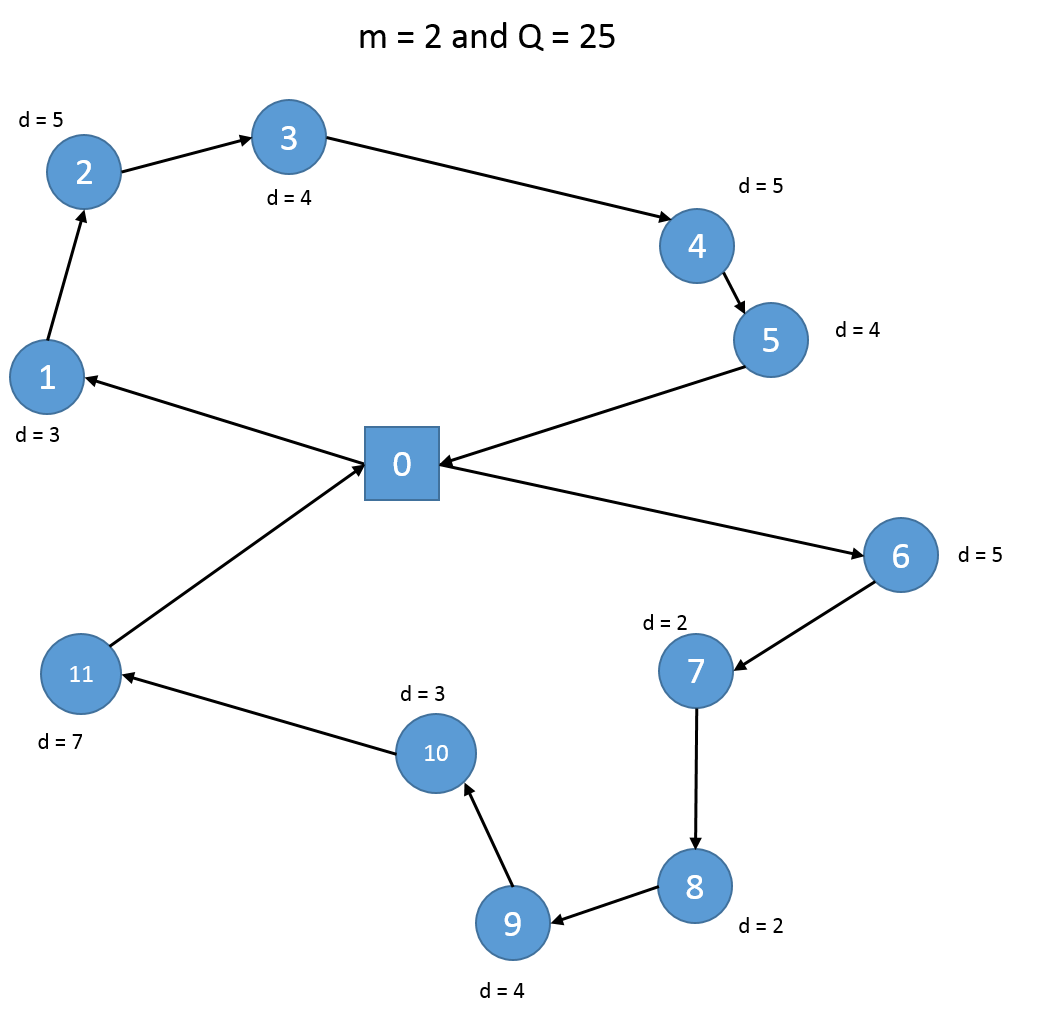
\includegraphics[width=0.6\linewidth]{Images/CVRP.png}
%\caption{Capacitated VRP}
%\label{fig:CVRP}
%\end{figure}
%\end{frame}
%
%\subsection{Generalized Vehicle Routing Problem}
%\begin{frame}
%\frametitle{Problem definition}
%\begin{figure}
%\centering
%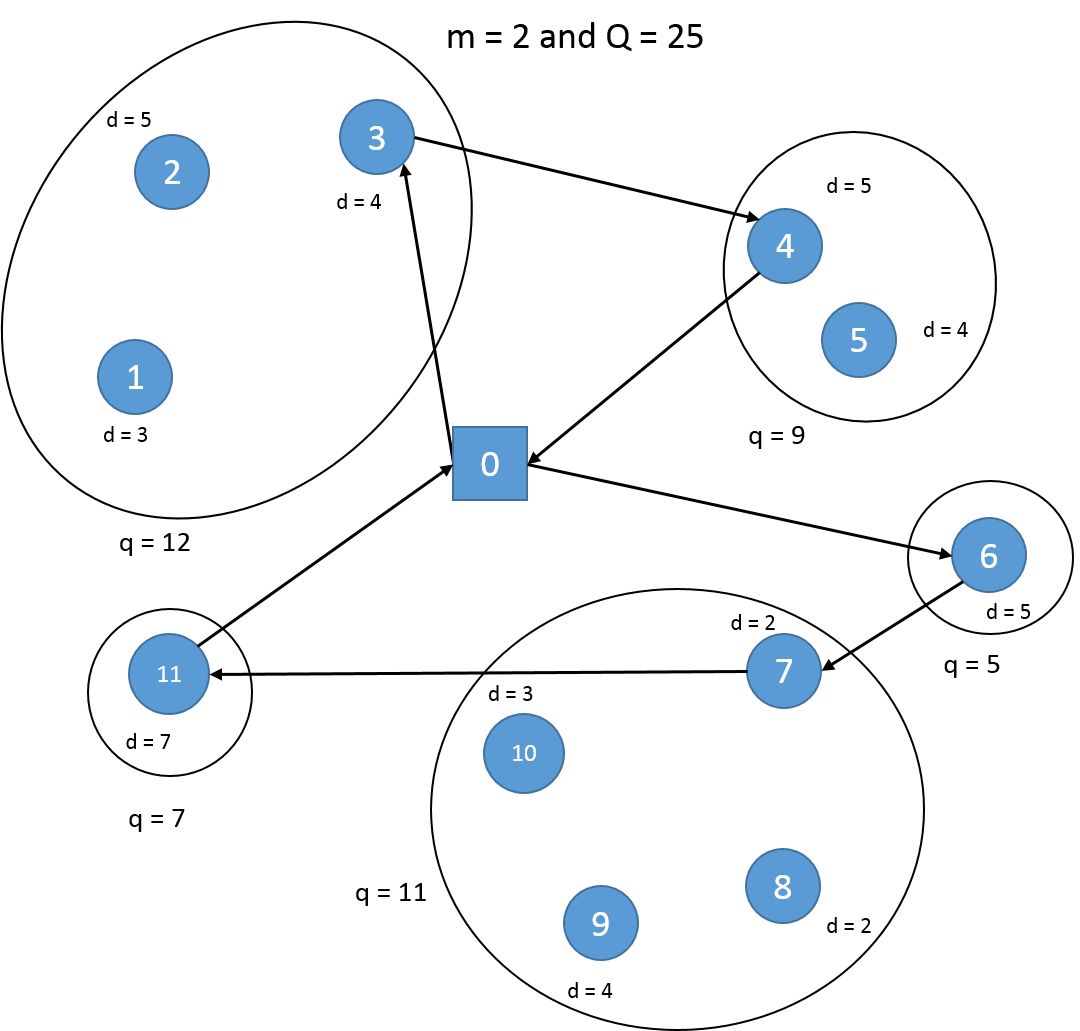
\includegraphics[height=0.6\linewidth]{Images/GVRP.png}
%\caption{Generalized VRP}
%\label{fig:GVRP}
%\end{figure}
%\end{frame}

\begin{frame}
\frametitle{\secname}
\begin{columns}[t,onlytextwidth]
\column{0.5\textwidth}

\begin{figure}
\centering
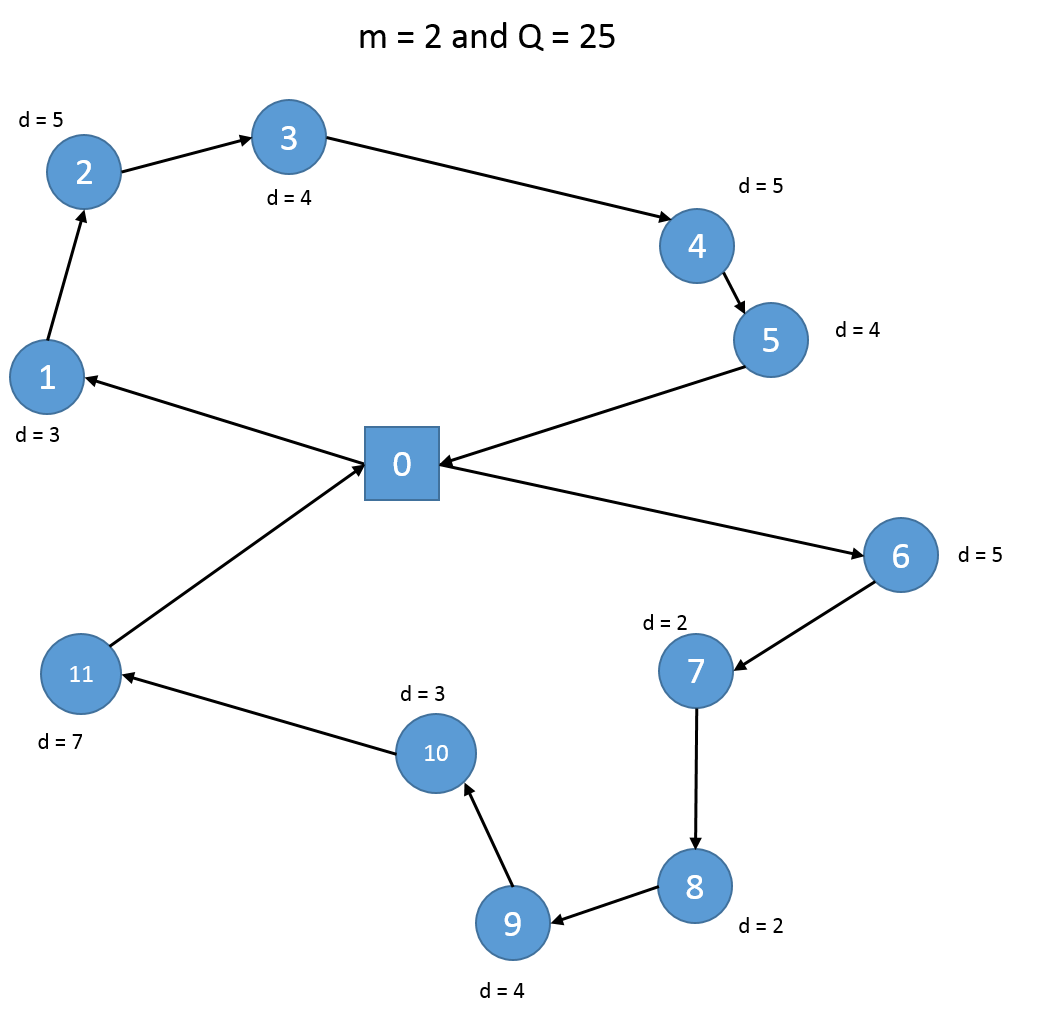
\includegraphics[width=\linewidth]{Images/CVRP.png}
\caption{Capacitated VRP}
\end{figure}

\column{0.5\textwidth}

\begin{figure}
\centering
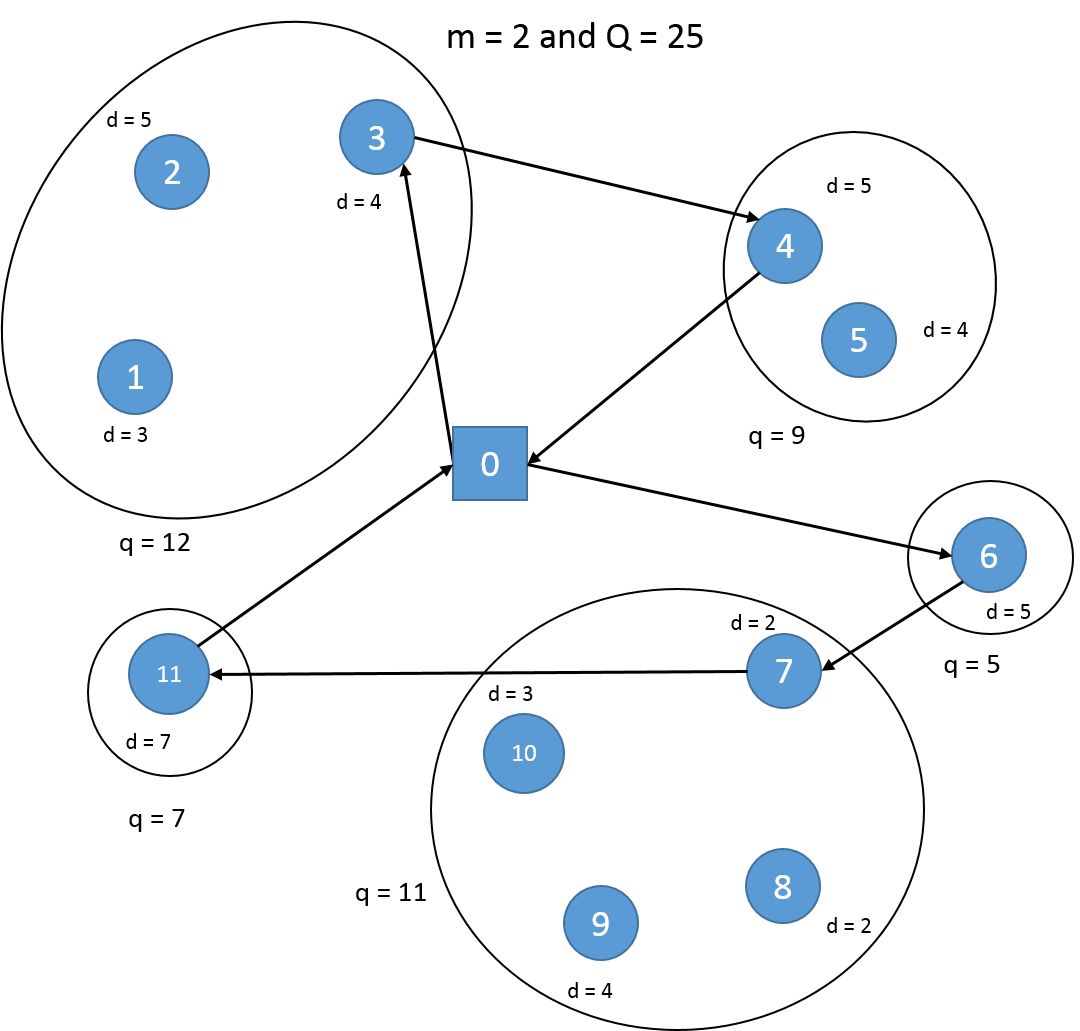
\includegraphics[width=\linewidth]{Images/GVRP.png}
\caption{Generalized VRP}
\end{figure}

\end{columns}

\end{frame}

%
\section{Solving the GVRP}
\subsection{General formulation}

\begin{frame}
\frametitle{\subsecname}
\textbf{Variables}
    \begin{align*}
    &x_{ij}= 
\begin{cases}
    1 & \text{if arc $(i,j)$ is included in the tour of a vehicle,  } \\
    0,              & \text{otherwise}
\end{cases} \\
    &w_{pr}= 
\begin{cases}
    1 & \text{if there is a path from cluster $V_p$ to cluster $V_r$,  }   \\
    0,              & \text{otherwise}
\end{cases}
\end{align*}

\textbf{Node-based} \\
$u_{p}$: load of a vehicle just after leaving the cluster $V_p$,  $p \ne 0$, $p \in K$

\textbf{Flow-based}\\
$y_{pr}$: amount of goods delivered by vehicle just after leaving the cluster $V_p$ if the vehicle goes from the cluster $V_p$ to the cluster $V_r$

\end{frame}

\begin{frame}
\frametitle{MILP formulation \footnotemark}
\begin{flalign*}
\text{min} \; &\sum_{i=1}^n \sum_{j=1}^n c_{ij} x_{ij}  \\
\text{s.t.} \; &\text{Cluster degree constraints} \\
			&\text{Cluster connectivity constraints}  \\
		  &\text{Capacity bounding constraints} \\	
		  &\text{Subtour elimination constraints} \\
		  &x_{i,j} \in \{0,1\}, \forall (i,j) \in A \nonumber
\end{flalign*}
\footnotetext[1]{\tiny Pop, P.~C., Kara, I., and Marc, A.~H.
\newblock New mathematical models of the generalized vehicle routing problem
  and extensions.
\newblock {\em Applied Mathematical Modelling}, 36(1):97 -- 107 (2012).}
\end{frame}

\begin{frame}
\frametitle{General constraints}
Constraints that are common between the two formulations:
\begin{itemize}
\item Cluster degree constraints: 
\begin{itemize}
\item exactly ONE outgoing arc to any other node belonging to other clusters 
\item exactly ONE incoming arc to a cluster from any other node belonging to other clusters
\item $m$ leaving arcs from and at most $m$ entering arcs to the depot ($= m$ or $\le m$)
\end{itemize}
\item Cluster connectivity constraints:
\begin{itemize}
\item entering and leaving nodes should be the same for each cluster
\item relation between $w_{pr}$ and $x_{ij}$
\end{itemize}
\end{itemize}
\end{frame}

\subsection{Node-based MILP formulation}
\begin{frame}
\frametitle{Node-based formulation}
$u_{p}$: load of a vehicle just after leaving the cluster $V_p$,  $p \ne 0$, $p \in K$
\begin{itemize}
\item Capacity bounding constraints
\begin{flalign*}
&u_p - \sum_{r \in K, r \ne p}q_r w_{rp} \ge q_p, \; p \ne 0, p \in K\\
&u_p + (Q - q_p) w_{0p} \le Q, \; p \ne 0, p \in K \\
&u_p + \sum_{r \in K, r \ne p} q_r w_{pr} \le Q, \; p \ne 0, p \in K 
\end{flalign*}
\item Subtour elimination constraints
\begin{equation*}
u_p - u_r + Q w_{pr} + (Q - q_p - q_r) w_{rp} \le Q - q_r, \;  p \ne r \ne 0; p, r \in K
\end{equation*}
\end{itemize}
\end{frame}

\subsection{Flow-based MILP formulation}
\begin{frame}
\frametitle{Flow-based formulation}
$y_{pr}$: amount of goods delivered by vehicle just after leaving the cluster $V_p$ if the vehicle goes from the cluster $V_p$ to the cluster $V_r$
\begin{itemize}
\item Capacity bounding constraints
\begin{flalign*}
&y_{rp} \le (Q - q_p) w_{rp}, \; r \ne p; r,p \in K  \\
&y_{rp} \ge q_r w_{rp}, \;  r \ne p; r, p \in K \\
&\sum_{p=1}^k y_{p0} =  \sum_{p=1}^k q_p \\
\end{flalign*}
\item Subtour elimination constraints
\begin{equation*}
\sum_{p=0}^k y_{rp} - \sum_{p=0}^k y_{pr} = q_r, \; r \ne 0; r,p \in K 
\end{equation*}
\end{itemize}
\end{frame}


\section{Test examples}

\begin{frame}
\frametitle{Test examples}
\begin{columns}[t,onlytextwidth]
\column{0.5\textwidth}

\begin{figure}
\centering
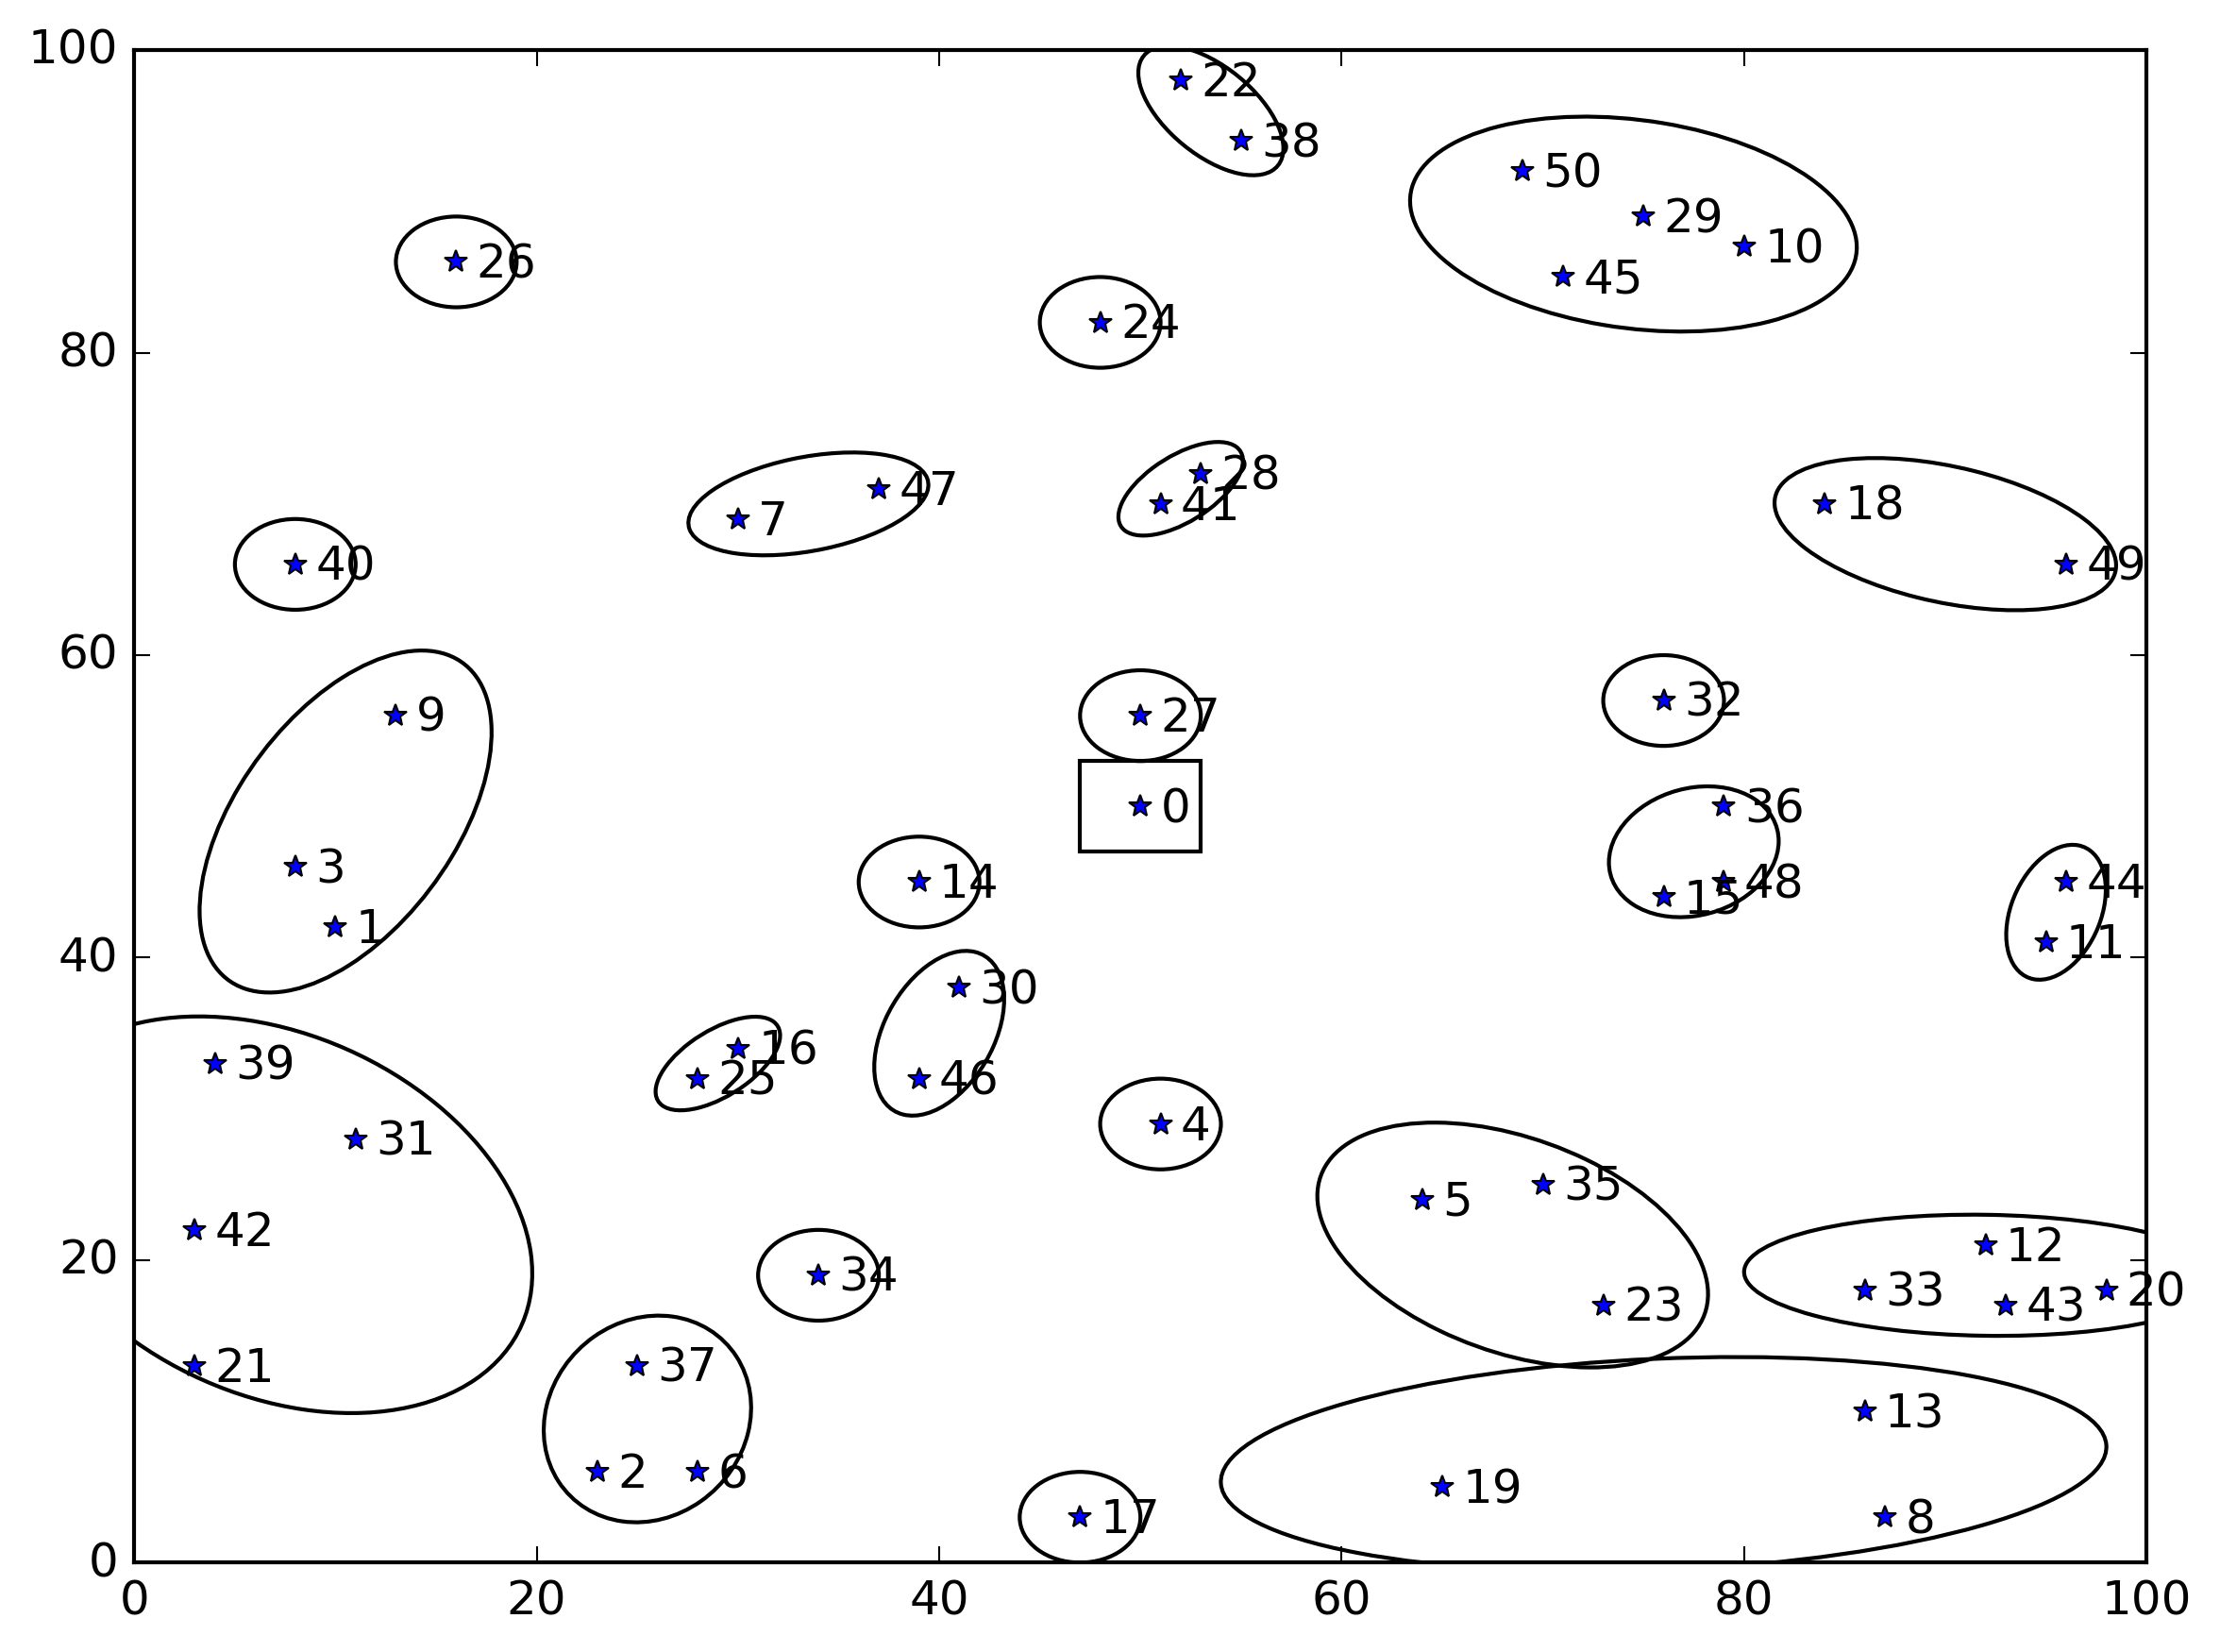
\includegraphics[width=\linewidth]{Images/GVRP_map.png}
\caption{\texttt{GVRP1} \footnotemark}
\end{figure}

\column{0.5\textwidth}

\begin{figure}
\centering
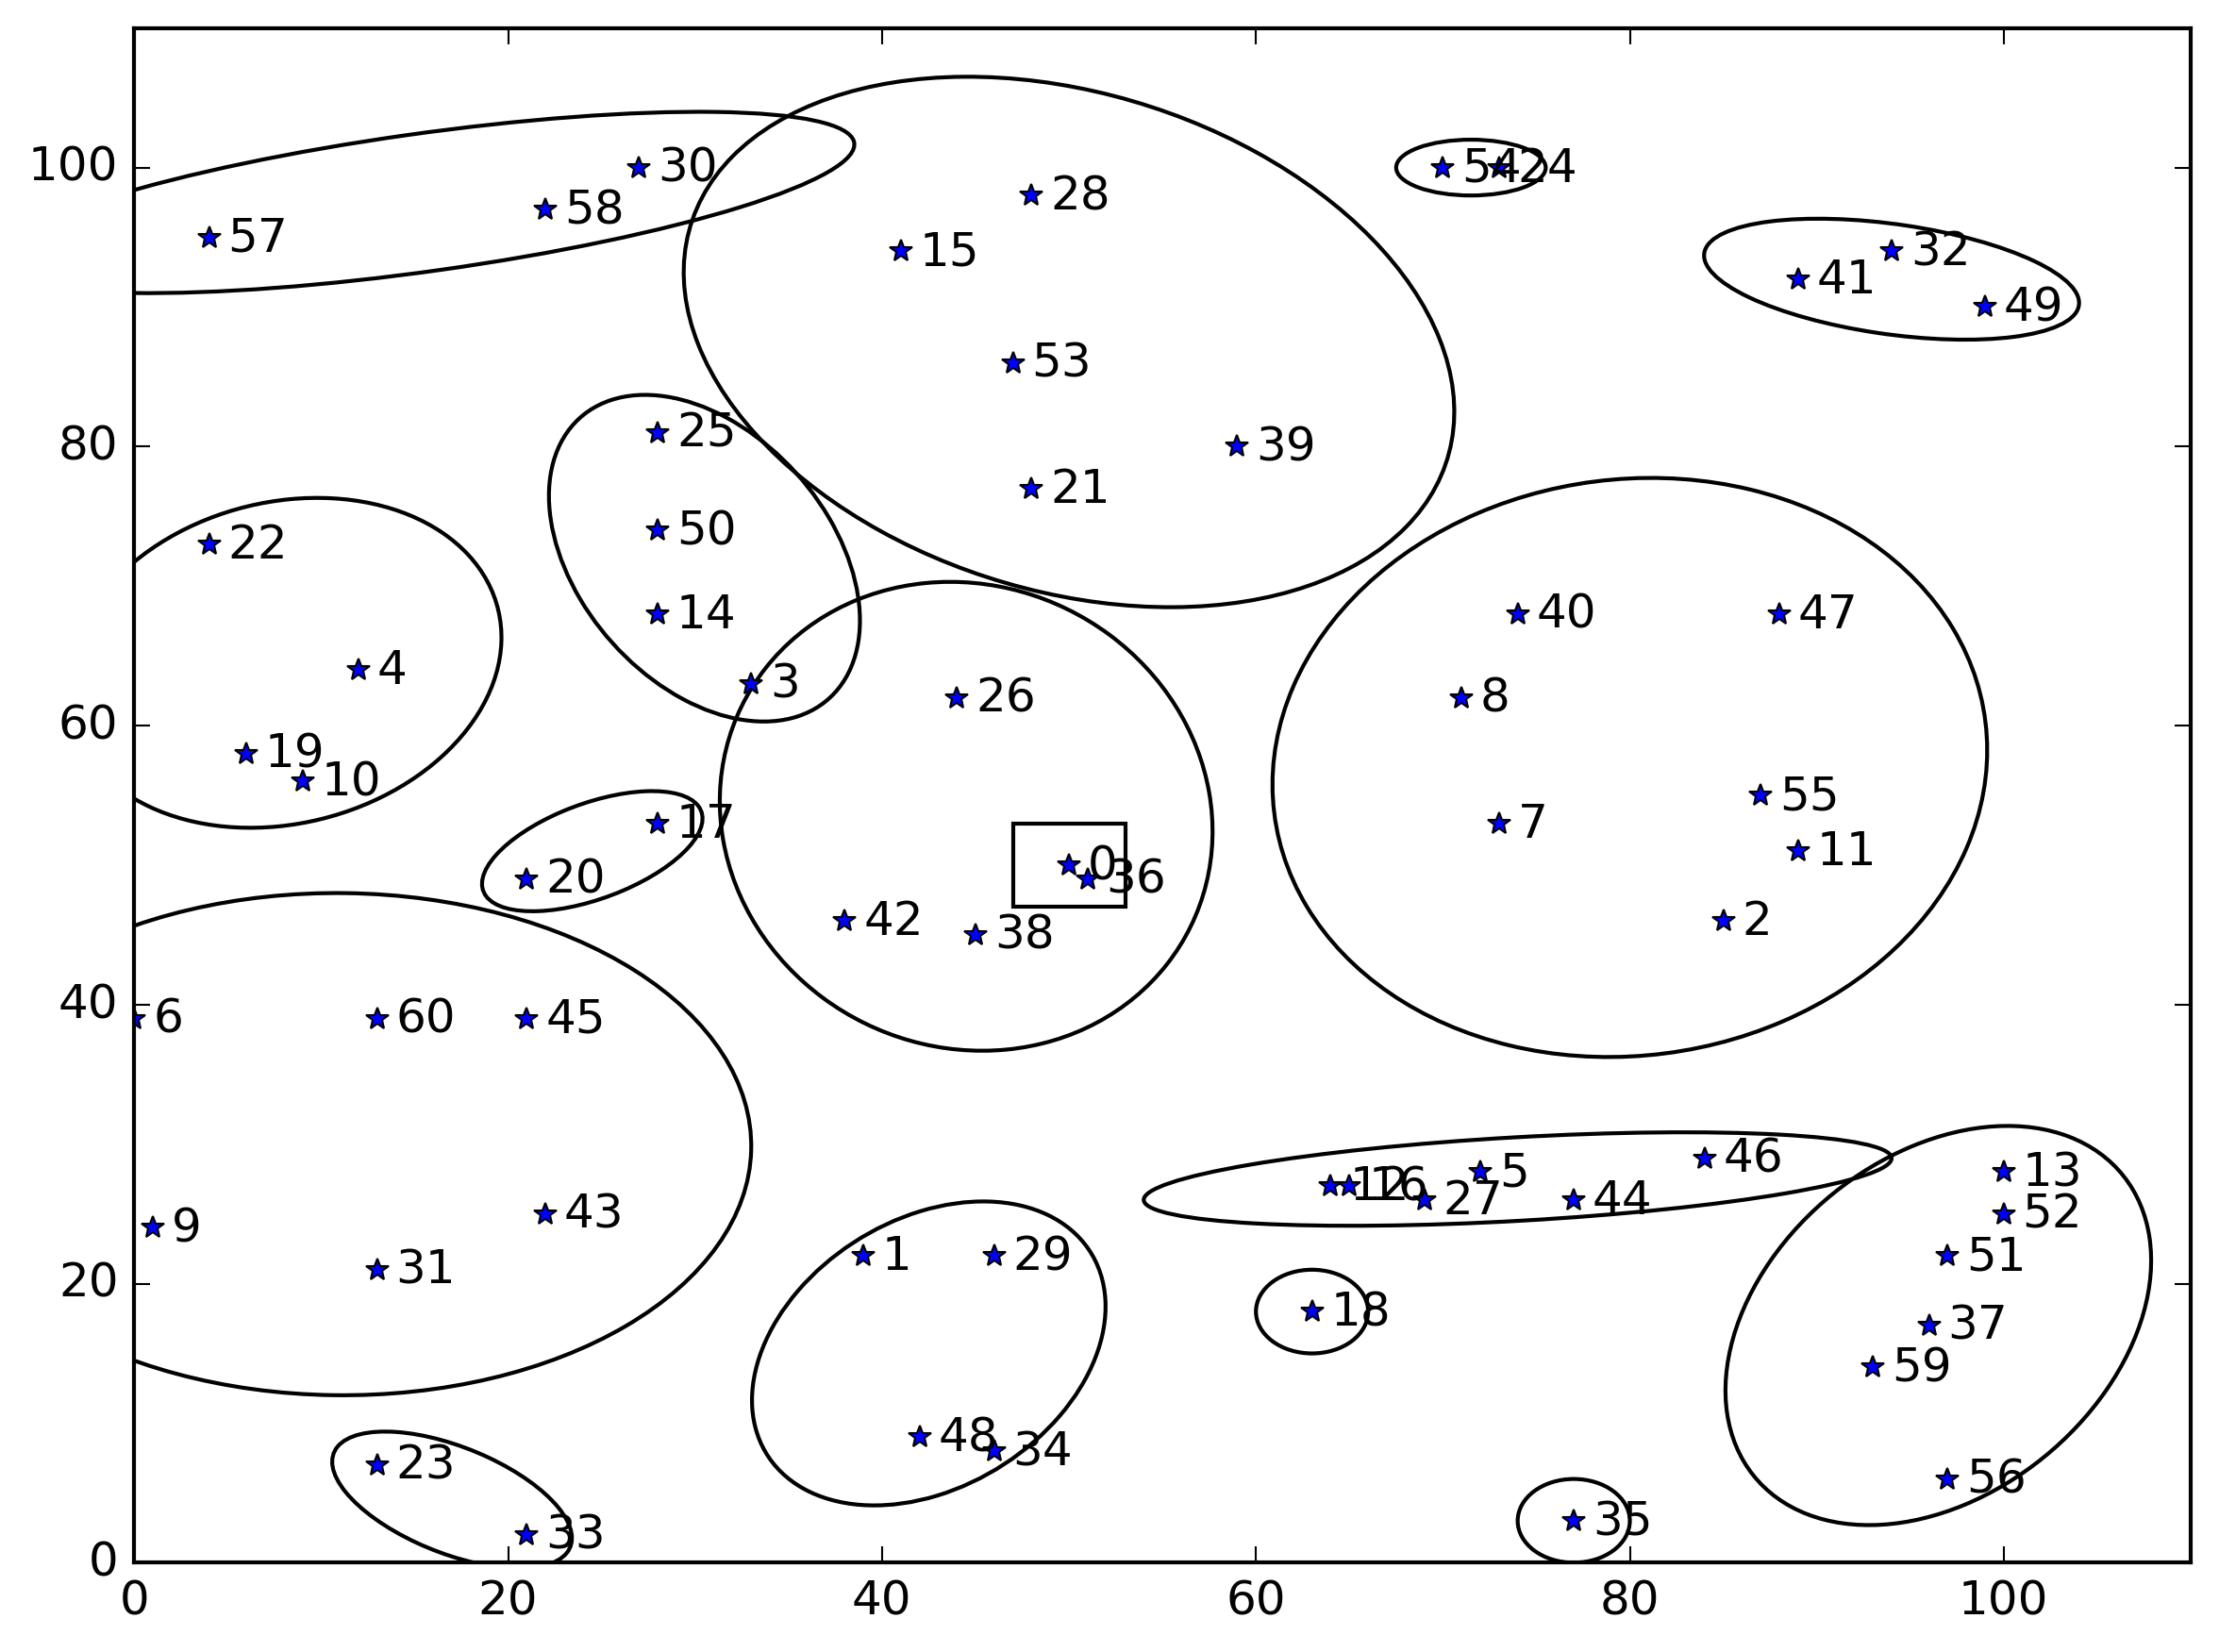
\includegraphics[width=\linewidth]{Images/GVRP2_map.png}
\caption{\texttt{GVRP2} \footnotemark}
\end{figure}

\end{columns}
\footnotetext[2]{\tiny Ghiani, G. and Improta, G. 
\newblock An effcient transformation of the generalized vehicle routing
problem. \newblock {\em European Journal of Operational Research}, 122(1):11 -- 17 (2000)}
\footnotetext[3]{\tiny
Kara, I. and Bekta\c{s}, T.
\newblock New mathematical models of the generalized vehicle routing problem
  and extensions.
\newblock {\em Proc. of the 5th EURO/INFORMS Joint International Meeting}
  (2003).
}
\end{frame}

\subsection{New test examples}
\begin{frame}
\frametitle{\subsecname}
\begin{itemize}
\item New test examples generated by clustering CVRP datasets from CVRPLIB \footnotemark
\item Simple clustering algo: K-means
\item Number of clusters such that max 4 customers in a cluster
\item Number of vehicles and capacities not maintained
\end{itemize}
\begin{columns}[t,onlytextwidth]
\column{.33\textwidth}

\begin{figure}
\centering
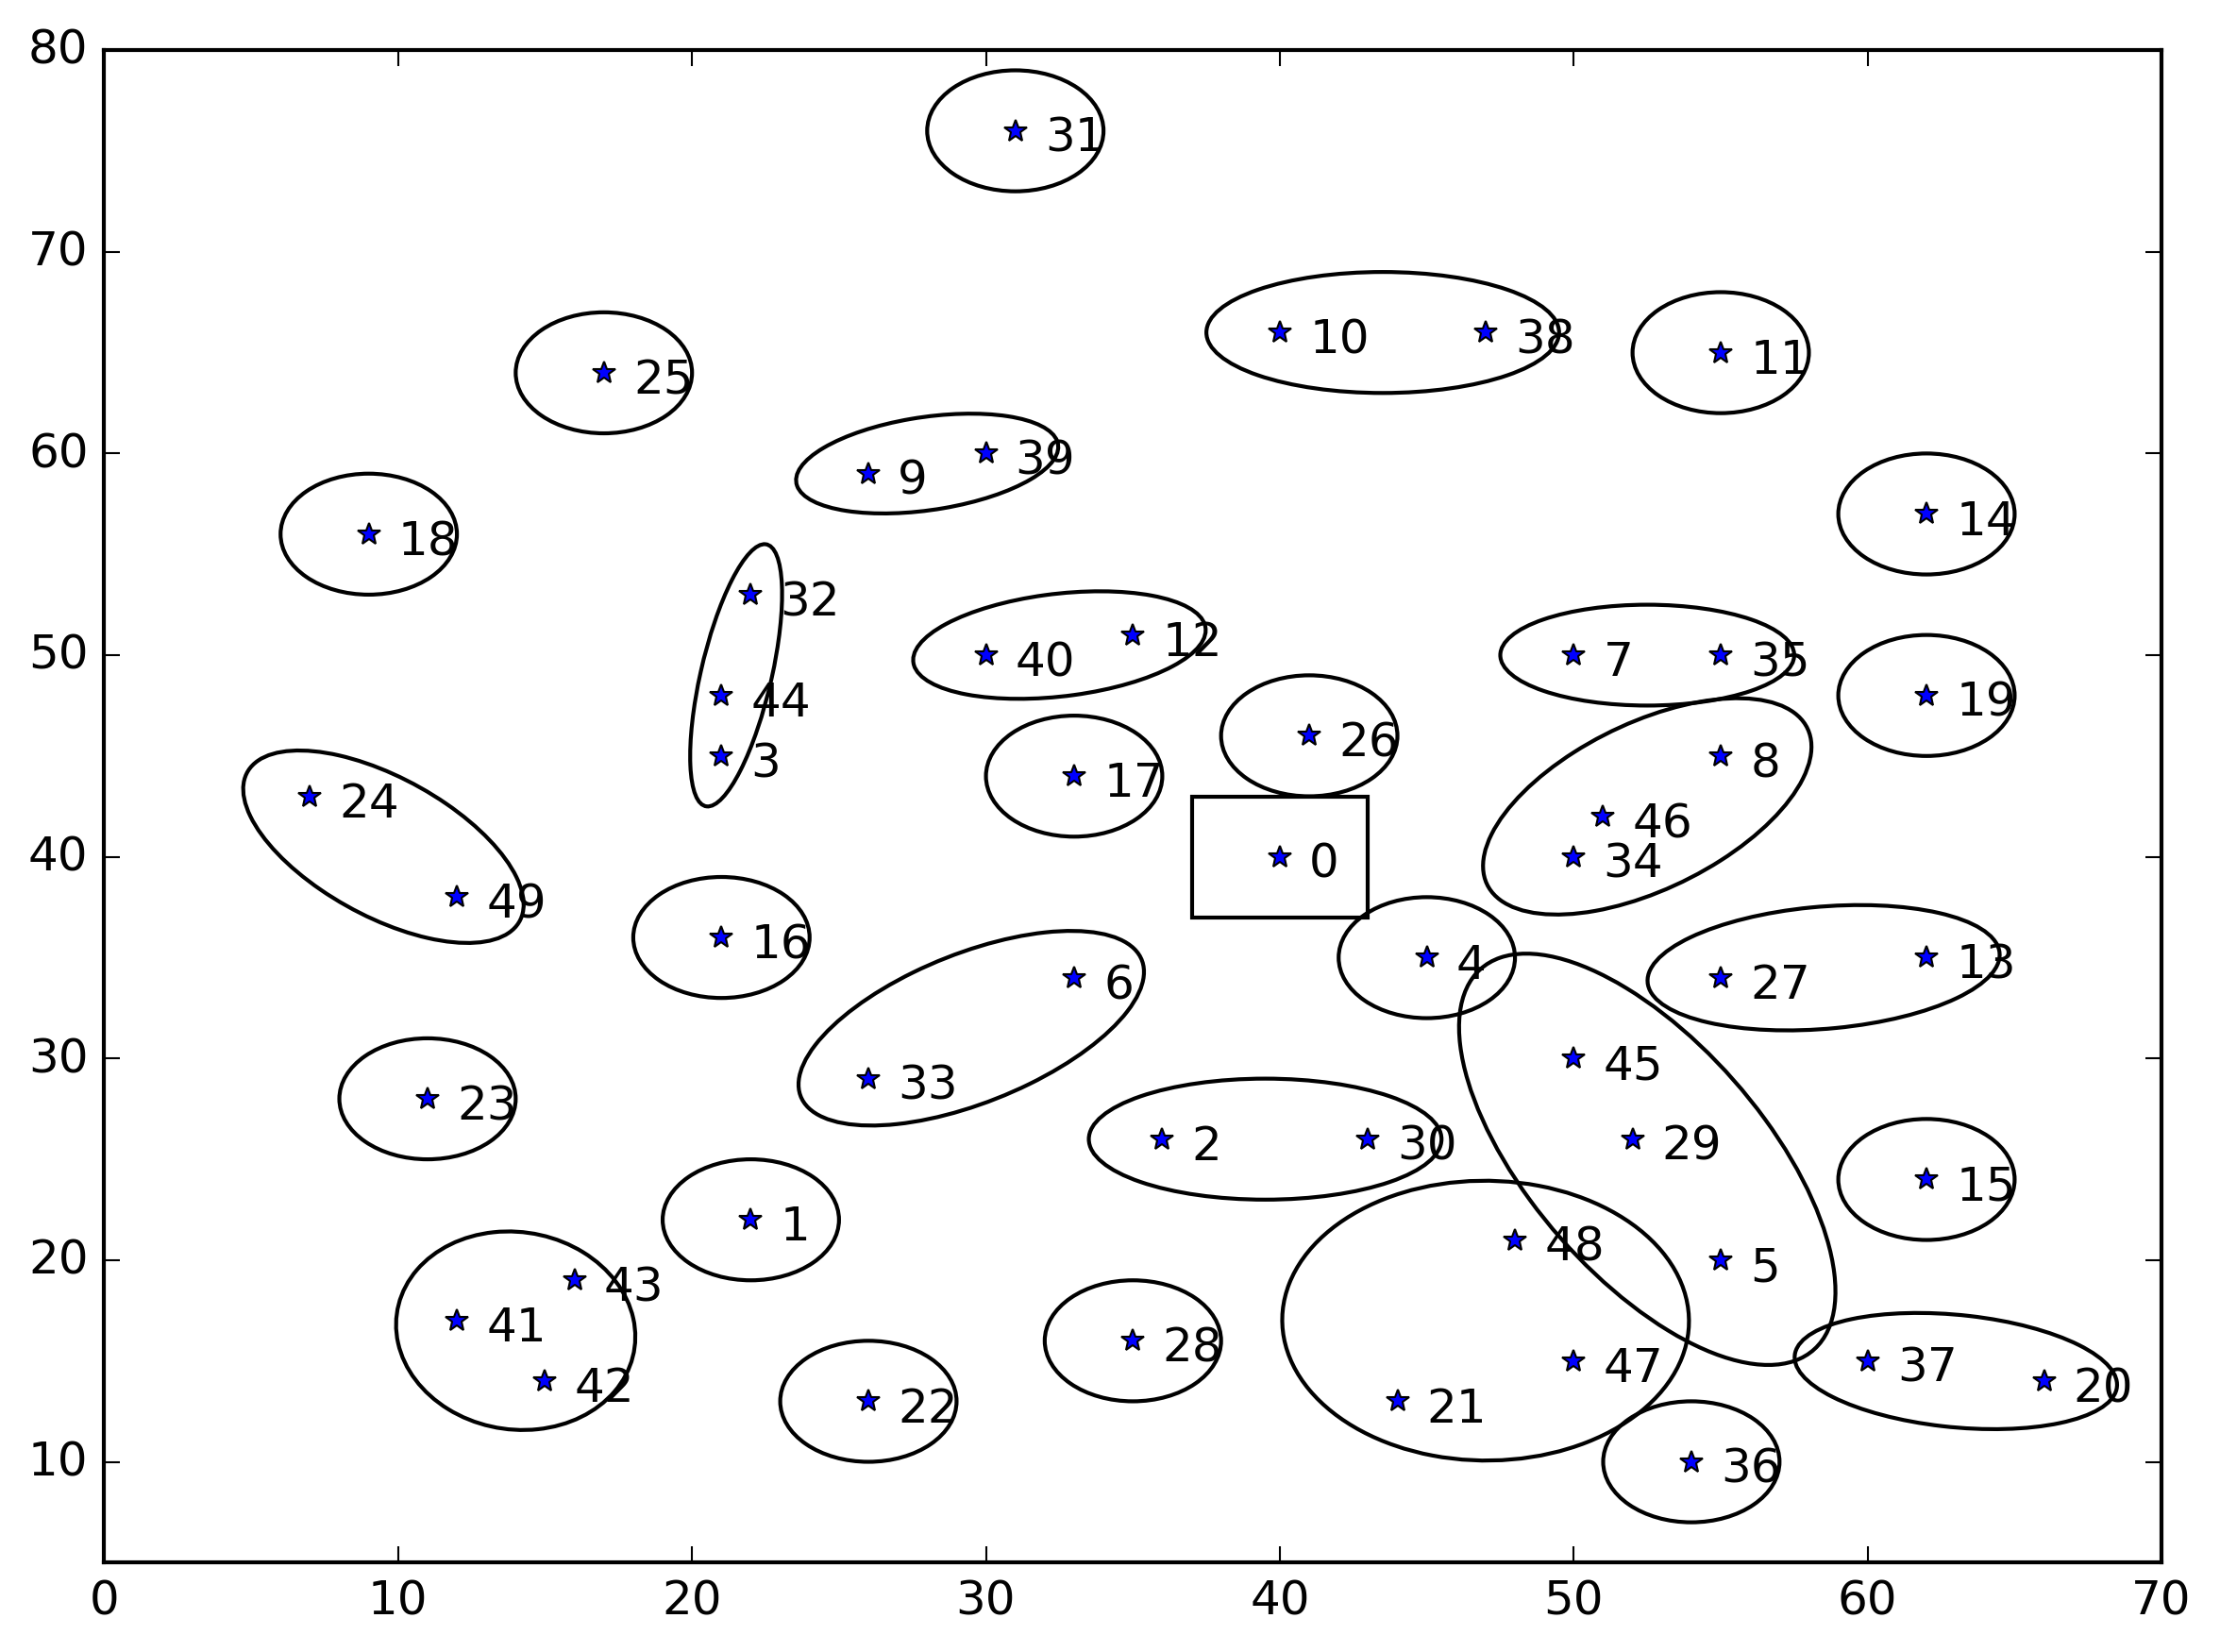
\includegraphics[width=\linewidth]{Images/P-n50-k10-c30_map.png}
\caption{\texttt{P-n50-k10}}
\end{figure}

\column{.33\textwidth}

\begin{figure}
\centering
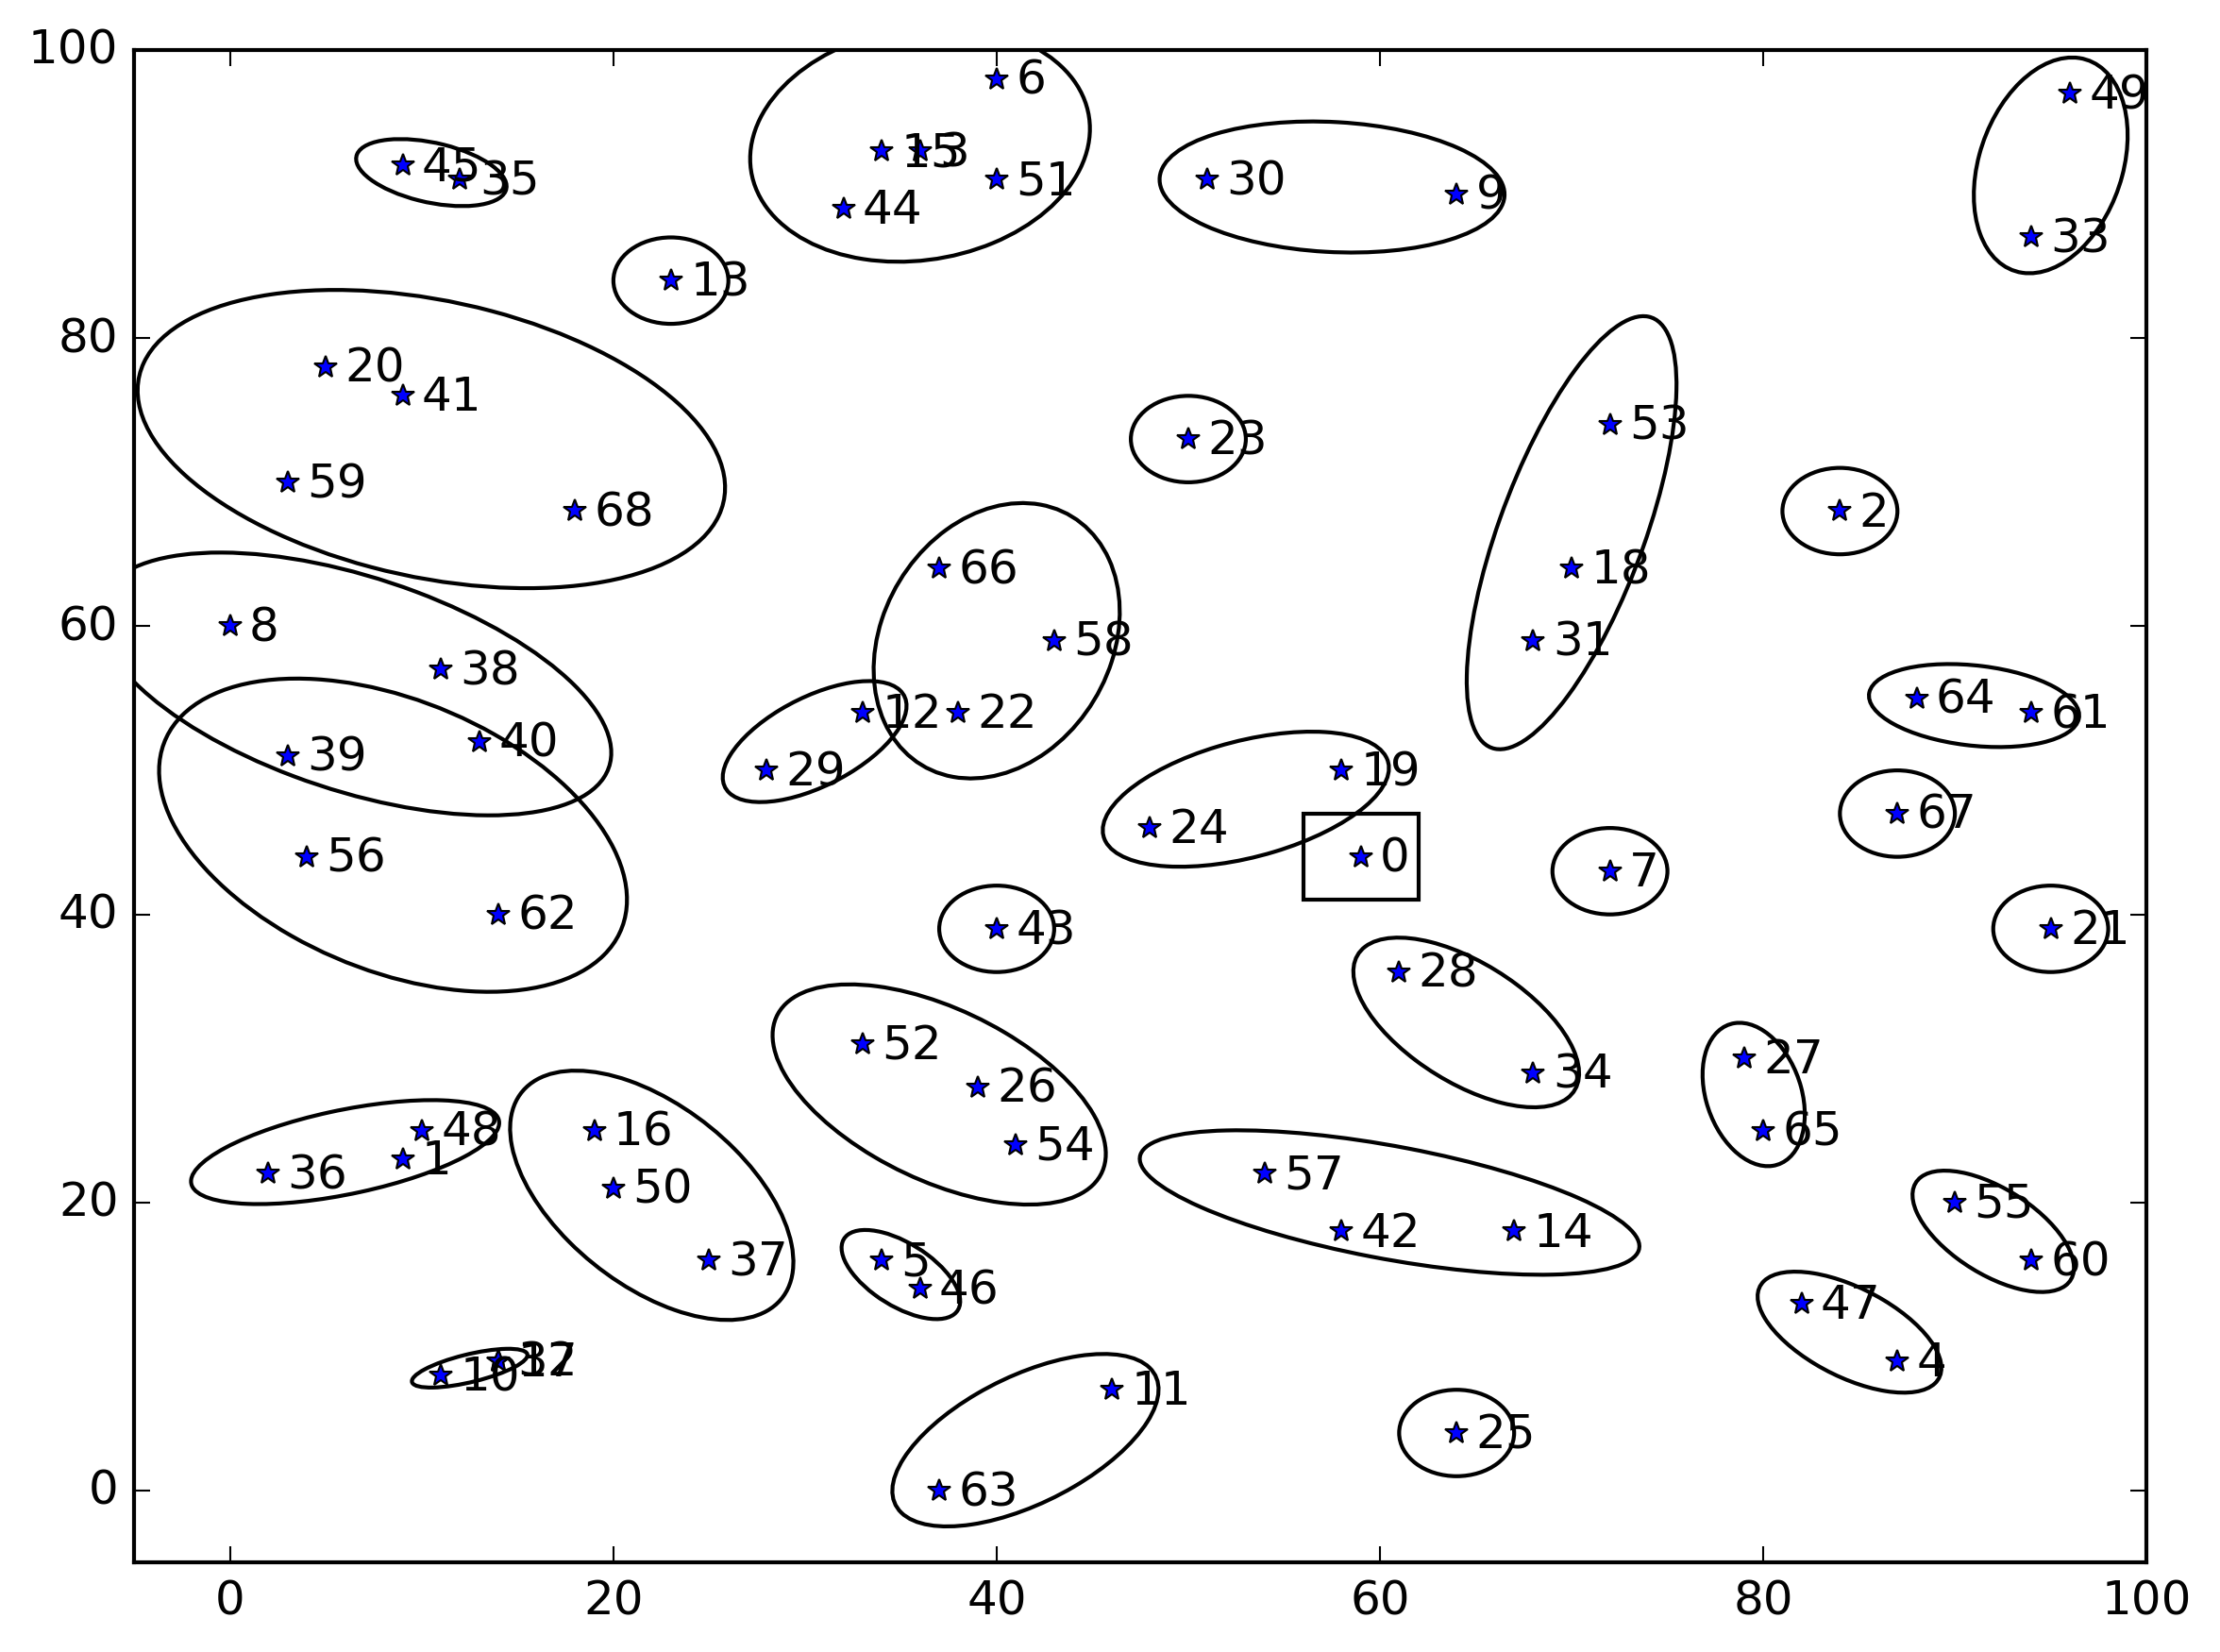
\includegraphics[width=\linewidth]{Images/A-n69-k9-c31_map.png}
\caption{\texttt{A-n69-k9}}
\end{figure}

\column{.33\textwidth}

\begin{figure}
\centering
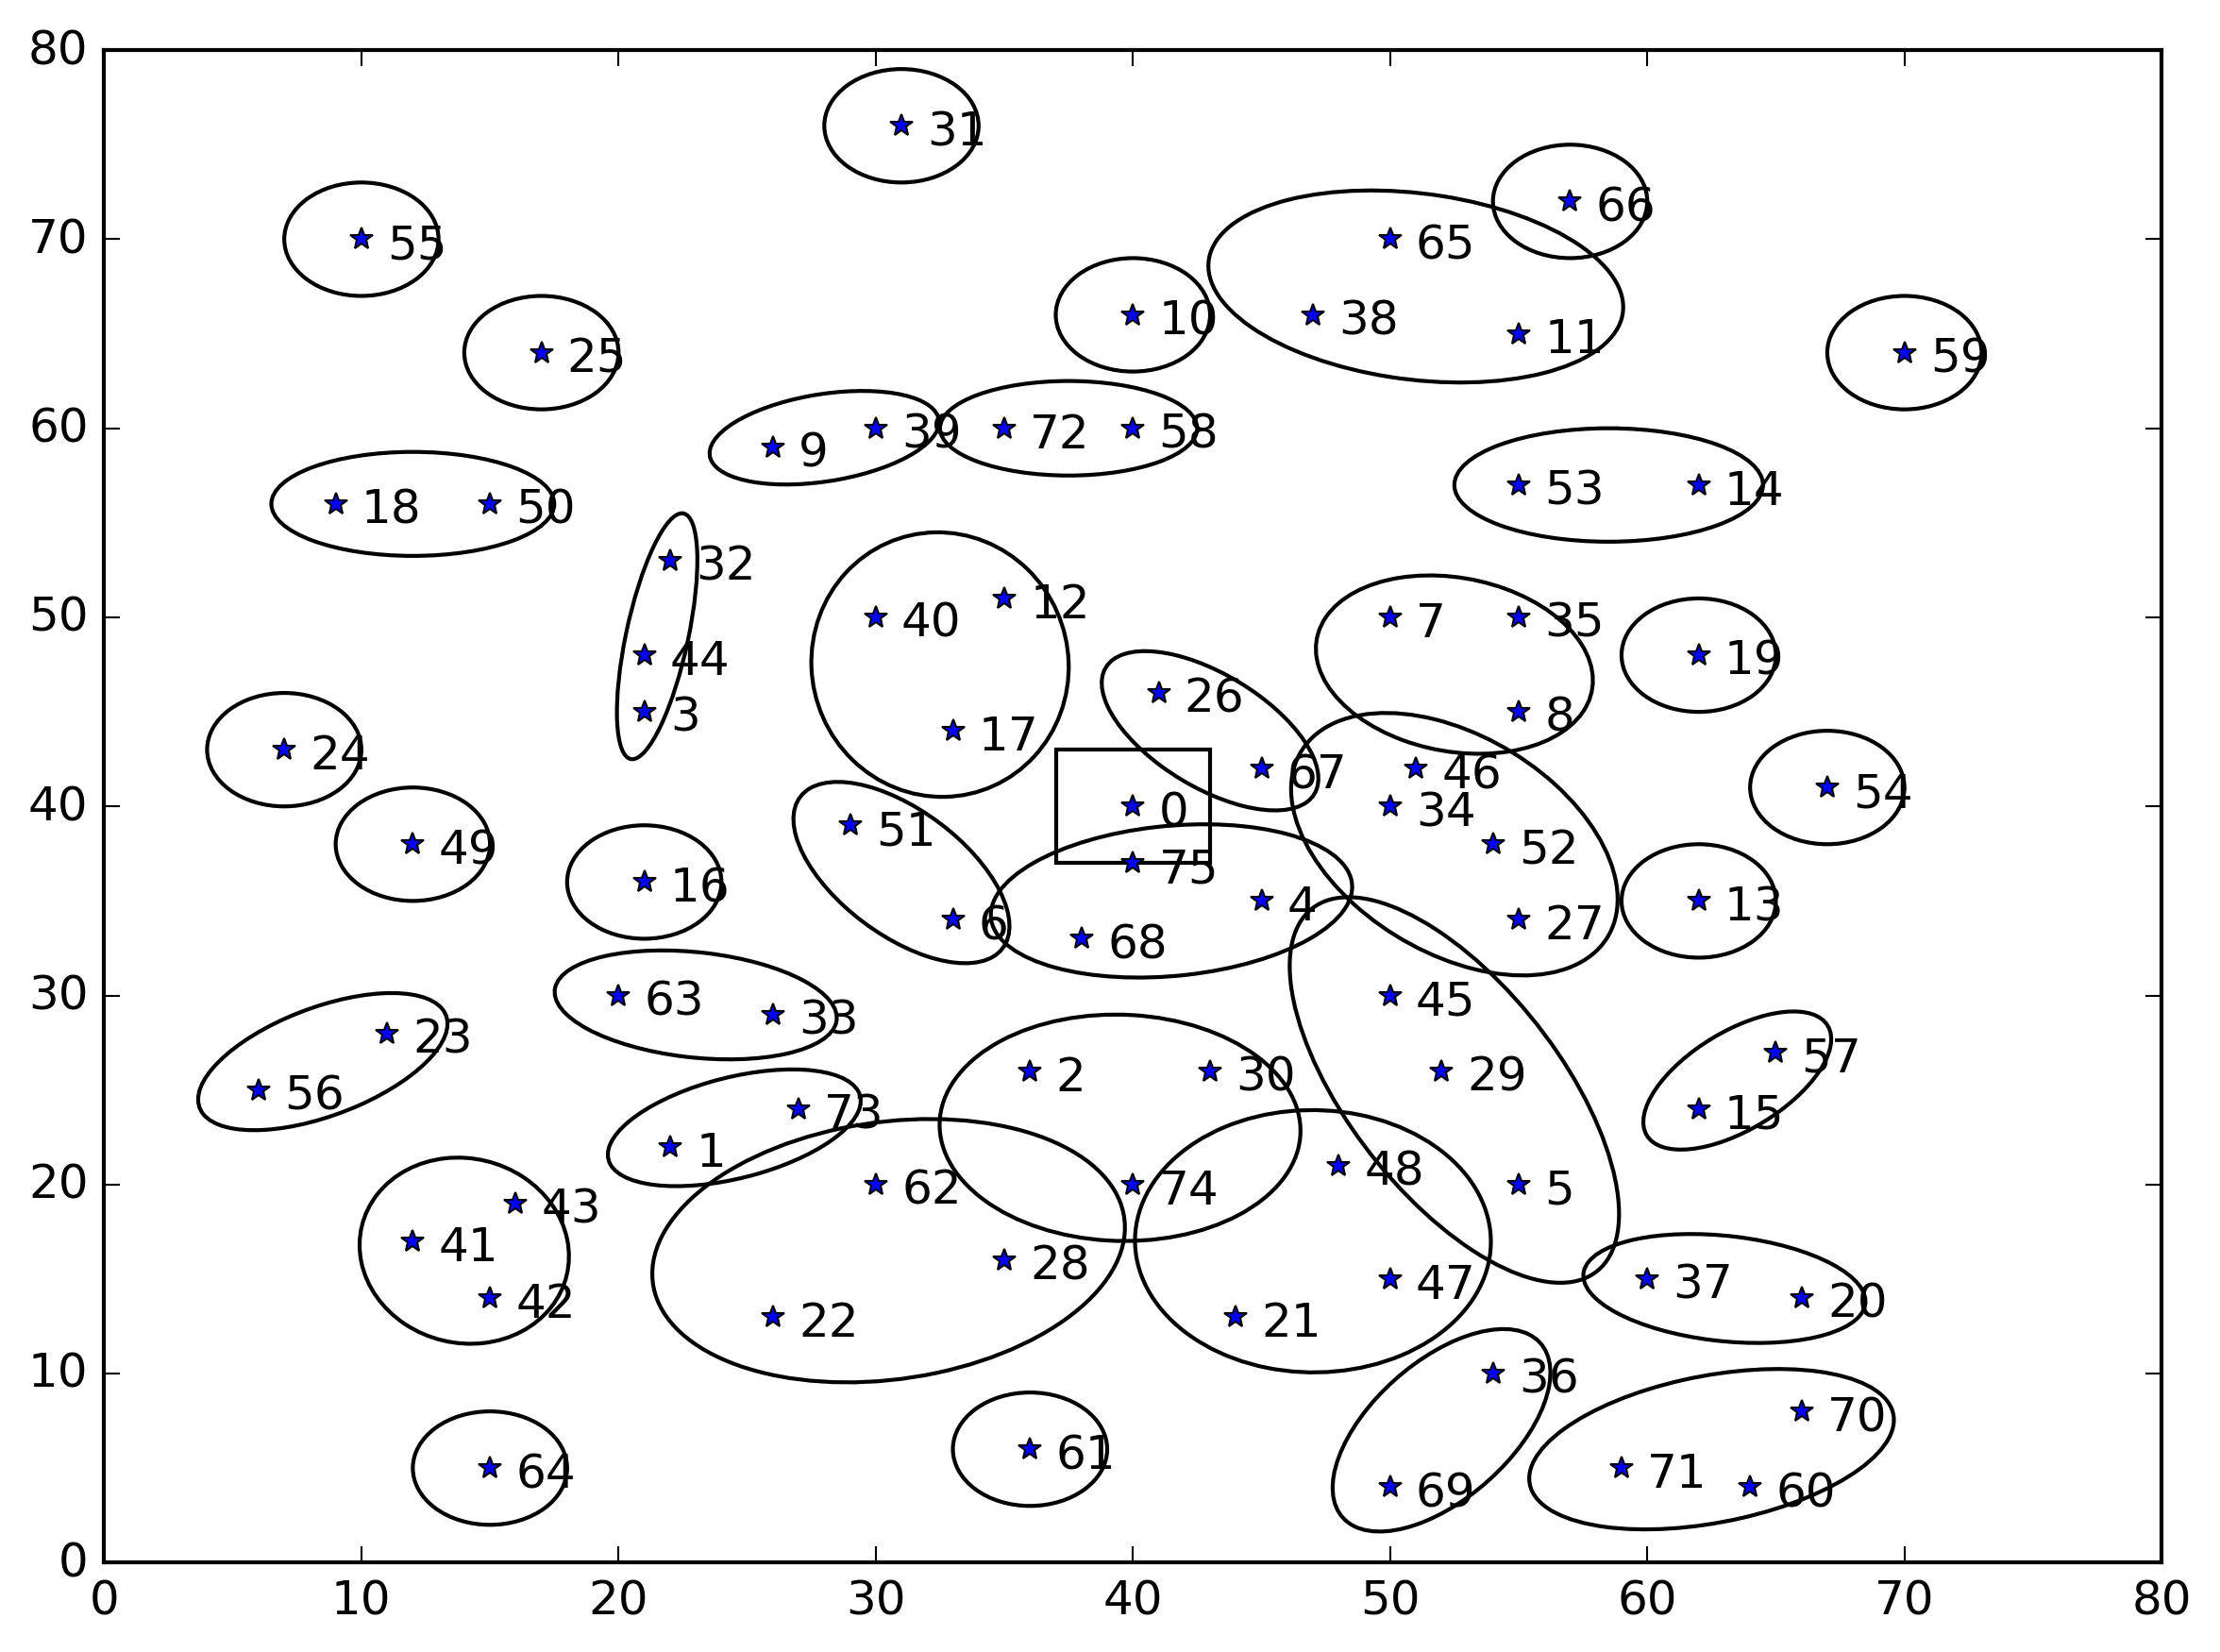
\includegraphics[width=\linewidth]{Images/P-n76-k5-c38_map.png}
\caption{\texttt{P-n76-k5}}
\end{figure}

\end{columns}
\footnotetext[4]{\url{http://vrp.atd-lab.inf.puc-rio.br/}}
\end{frame}


\section{Computational study}

\begin{frame}
\frametitle{Implementation}
\begin{itemize}
\item Node-based and flow-based formulations implemented using CPLEX/C++ API
\item Windows PC with an Intel i7 processor (2.90 GHz)
\item Optimal solutions found for \texttt{GVRP1}, \texttt{GVRP2}, \texttt{P-n50-k10}, \texttt{A-n69-k9} using flow-based formulation
\item \texttt{P-n76-k5} solved to 2.55\% relative gap
\end{itemize}
\end{frame}

\begin{frame}

\begin{columns}[t,onlytextwidth]
\column{0.11\textwidth}
\column{0.33\textwidth}

\begin{figure}
\centering
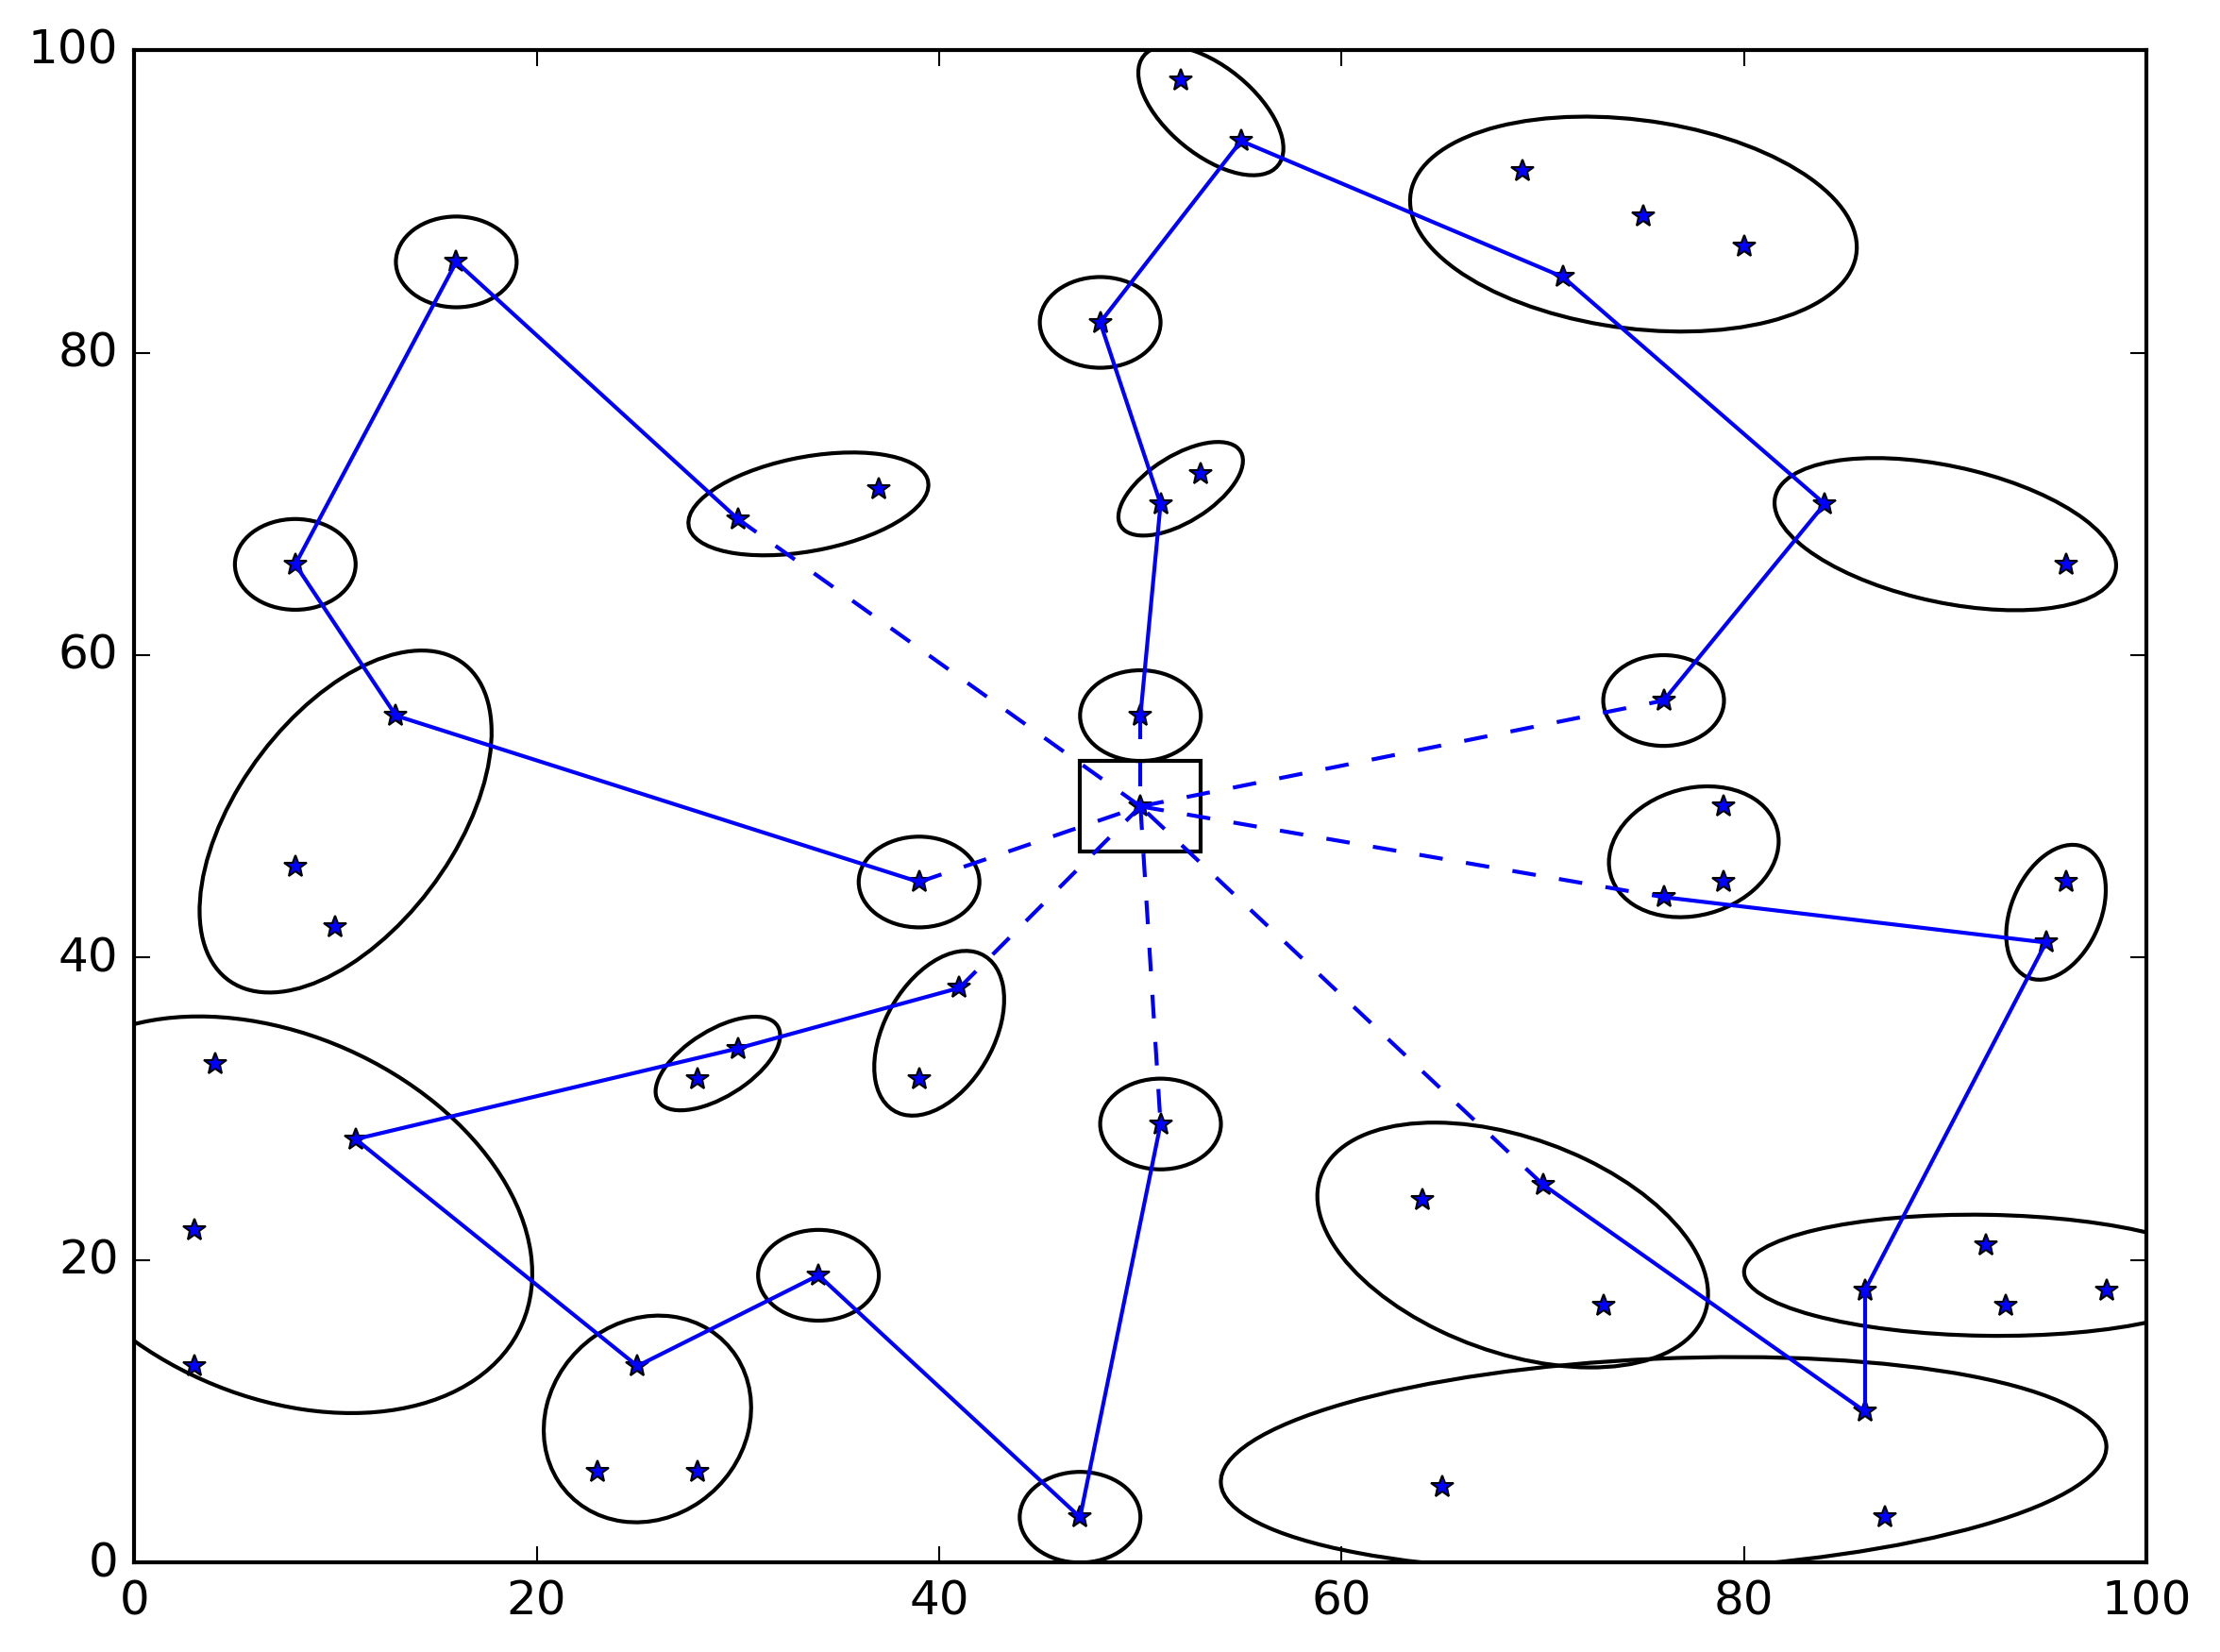
\includegraphics[width=\linewidth]{Images/GVRP_flow_n51_k25_m4_Q15_TL60_map.png}
\caption{\texttt{GVRP1}}
\end{figure}

\column{0.33\textwidth}

\begin{figure}
\centering
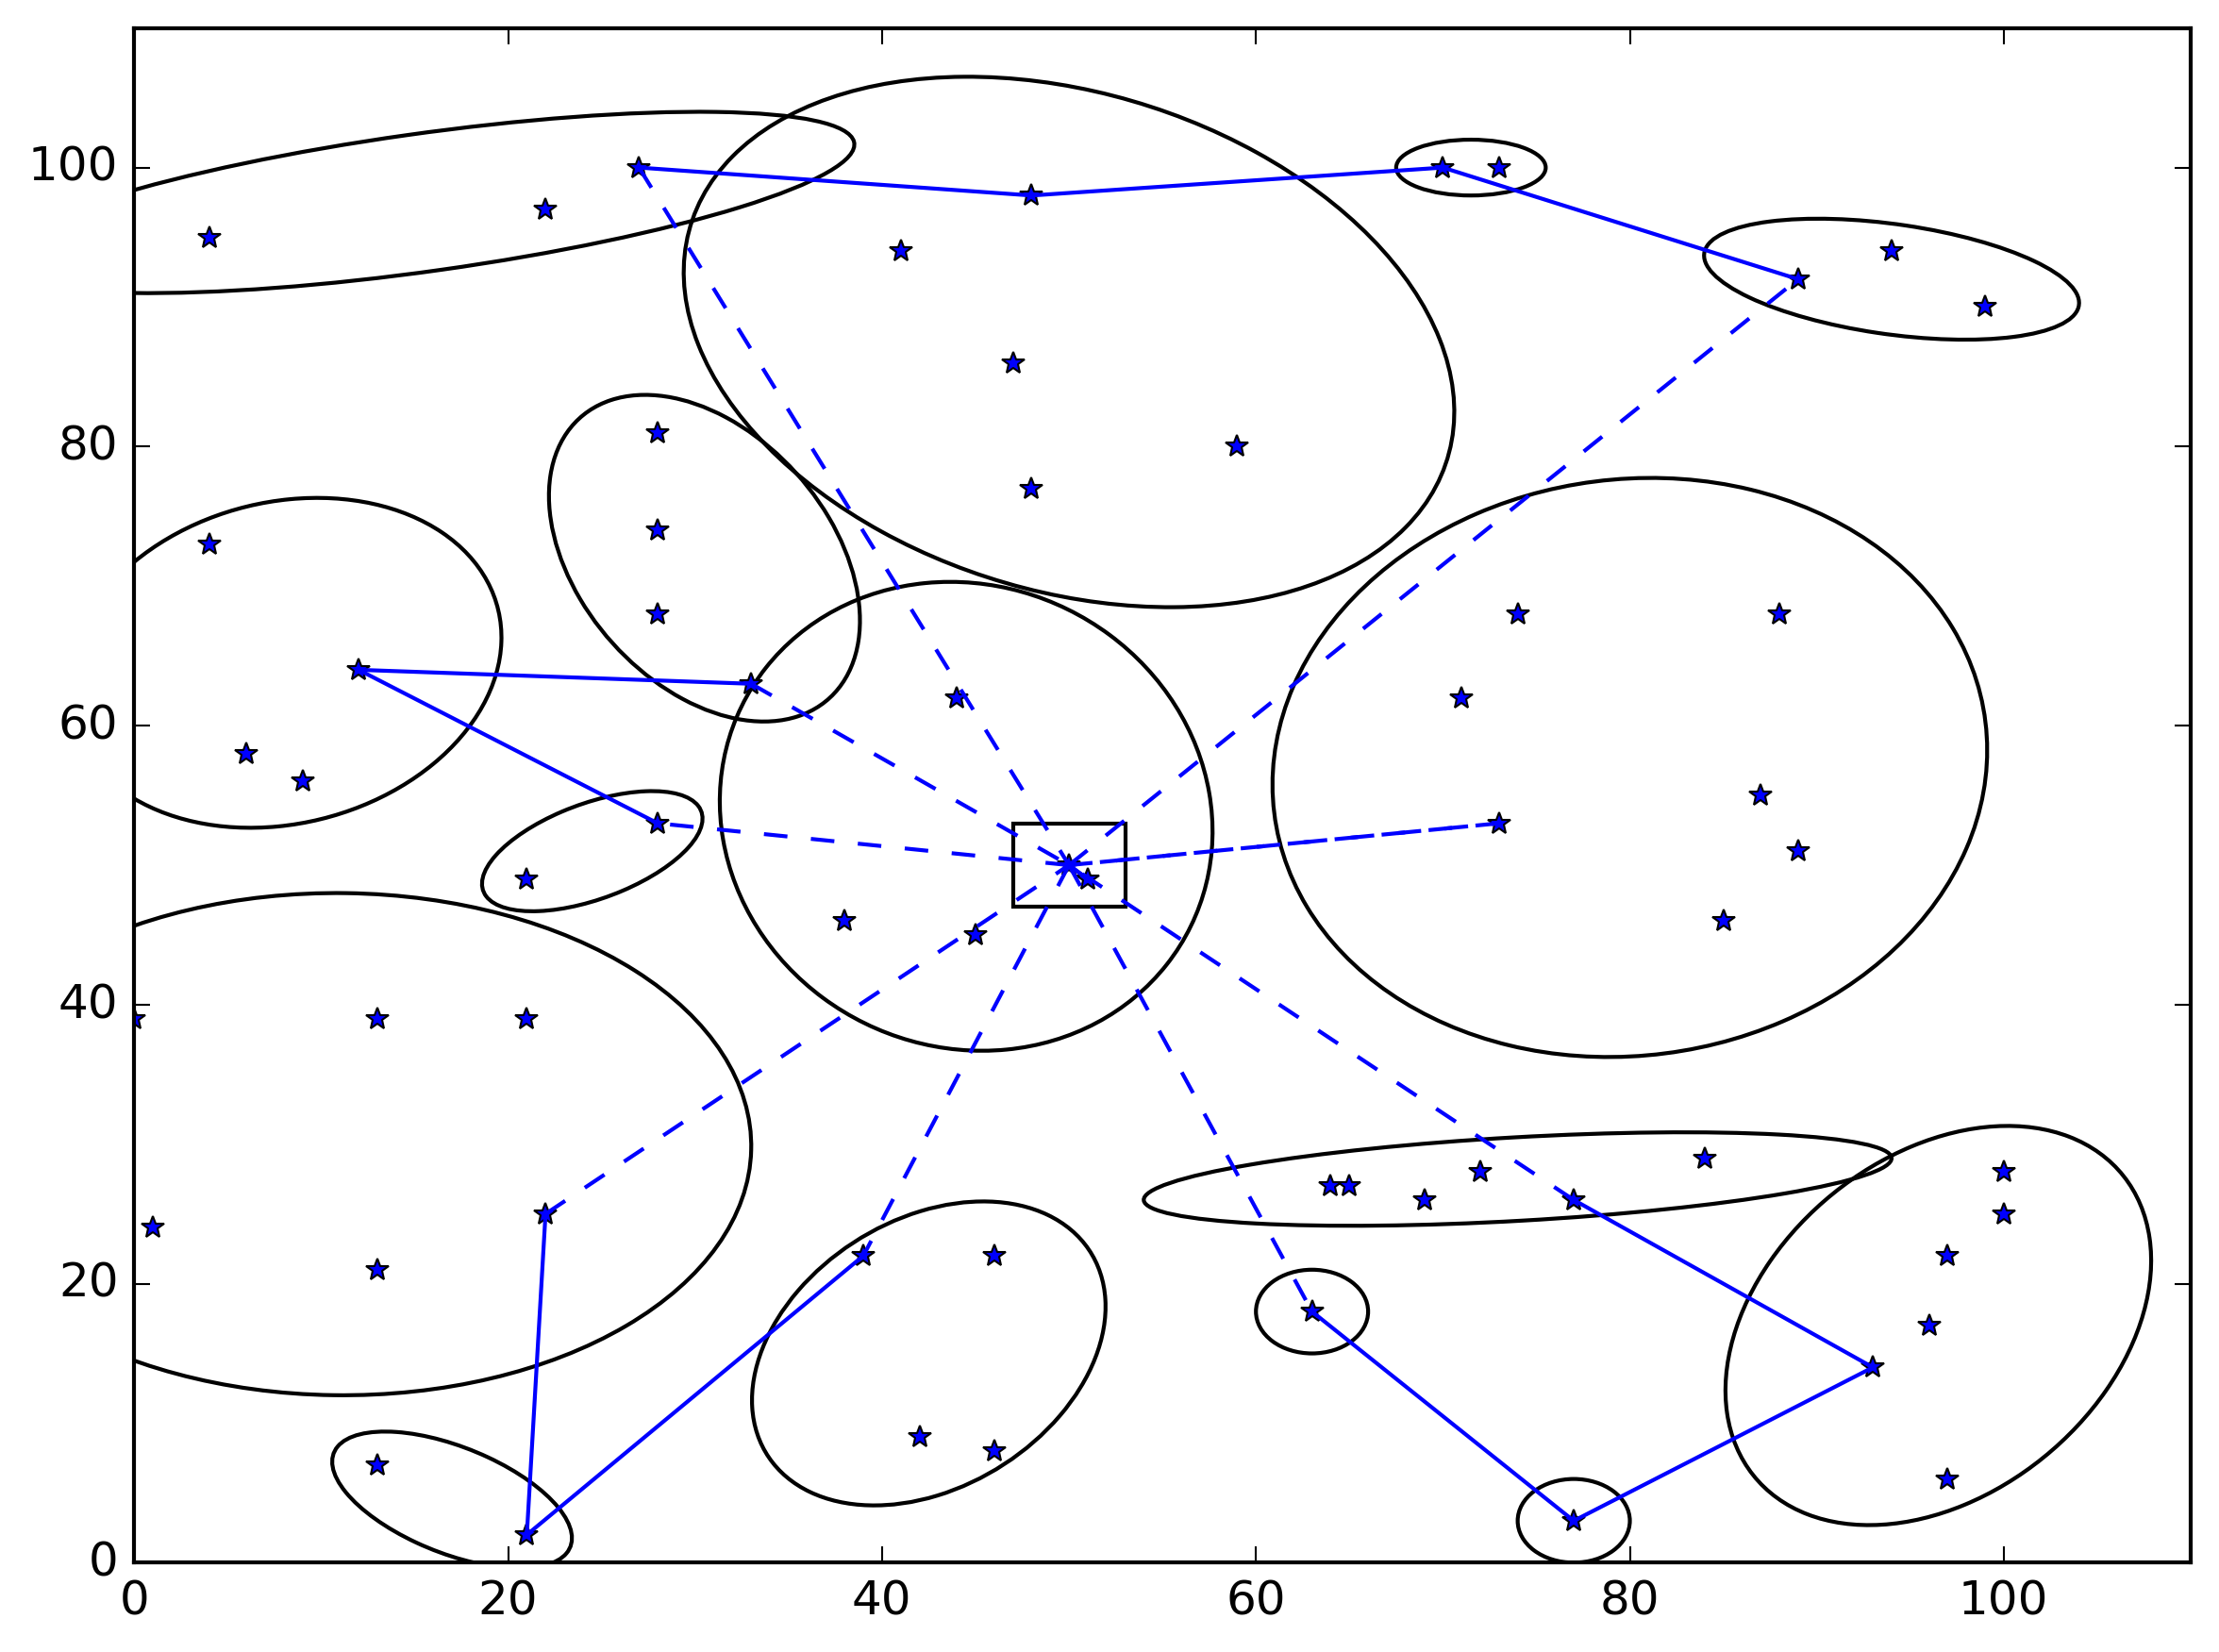
\includegraphics[width=\linewidth]{Images/GVRP2_flow_n61_k17_m6_Q15_TL10_map.png}
\caption{\texttt{GVRP2}}
\end{figure}
\column{0.11\textwidth}
\end{columns}

\begin{columns}[t,onlytextwidth]
\column{.33\textwidth}
\begin{figure}
\centering
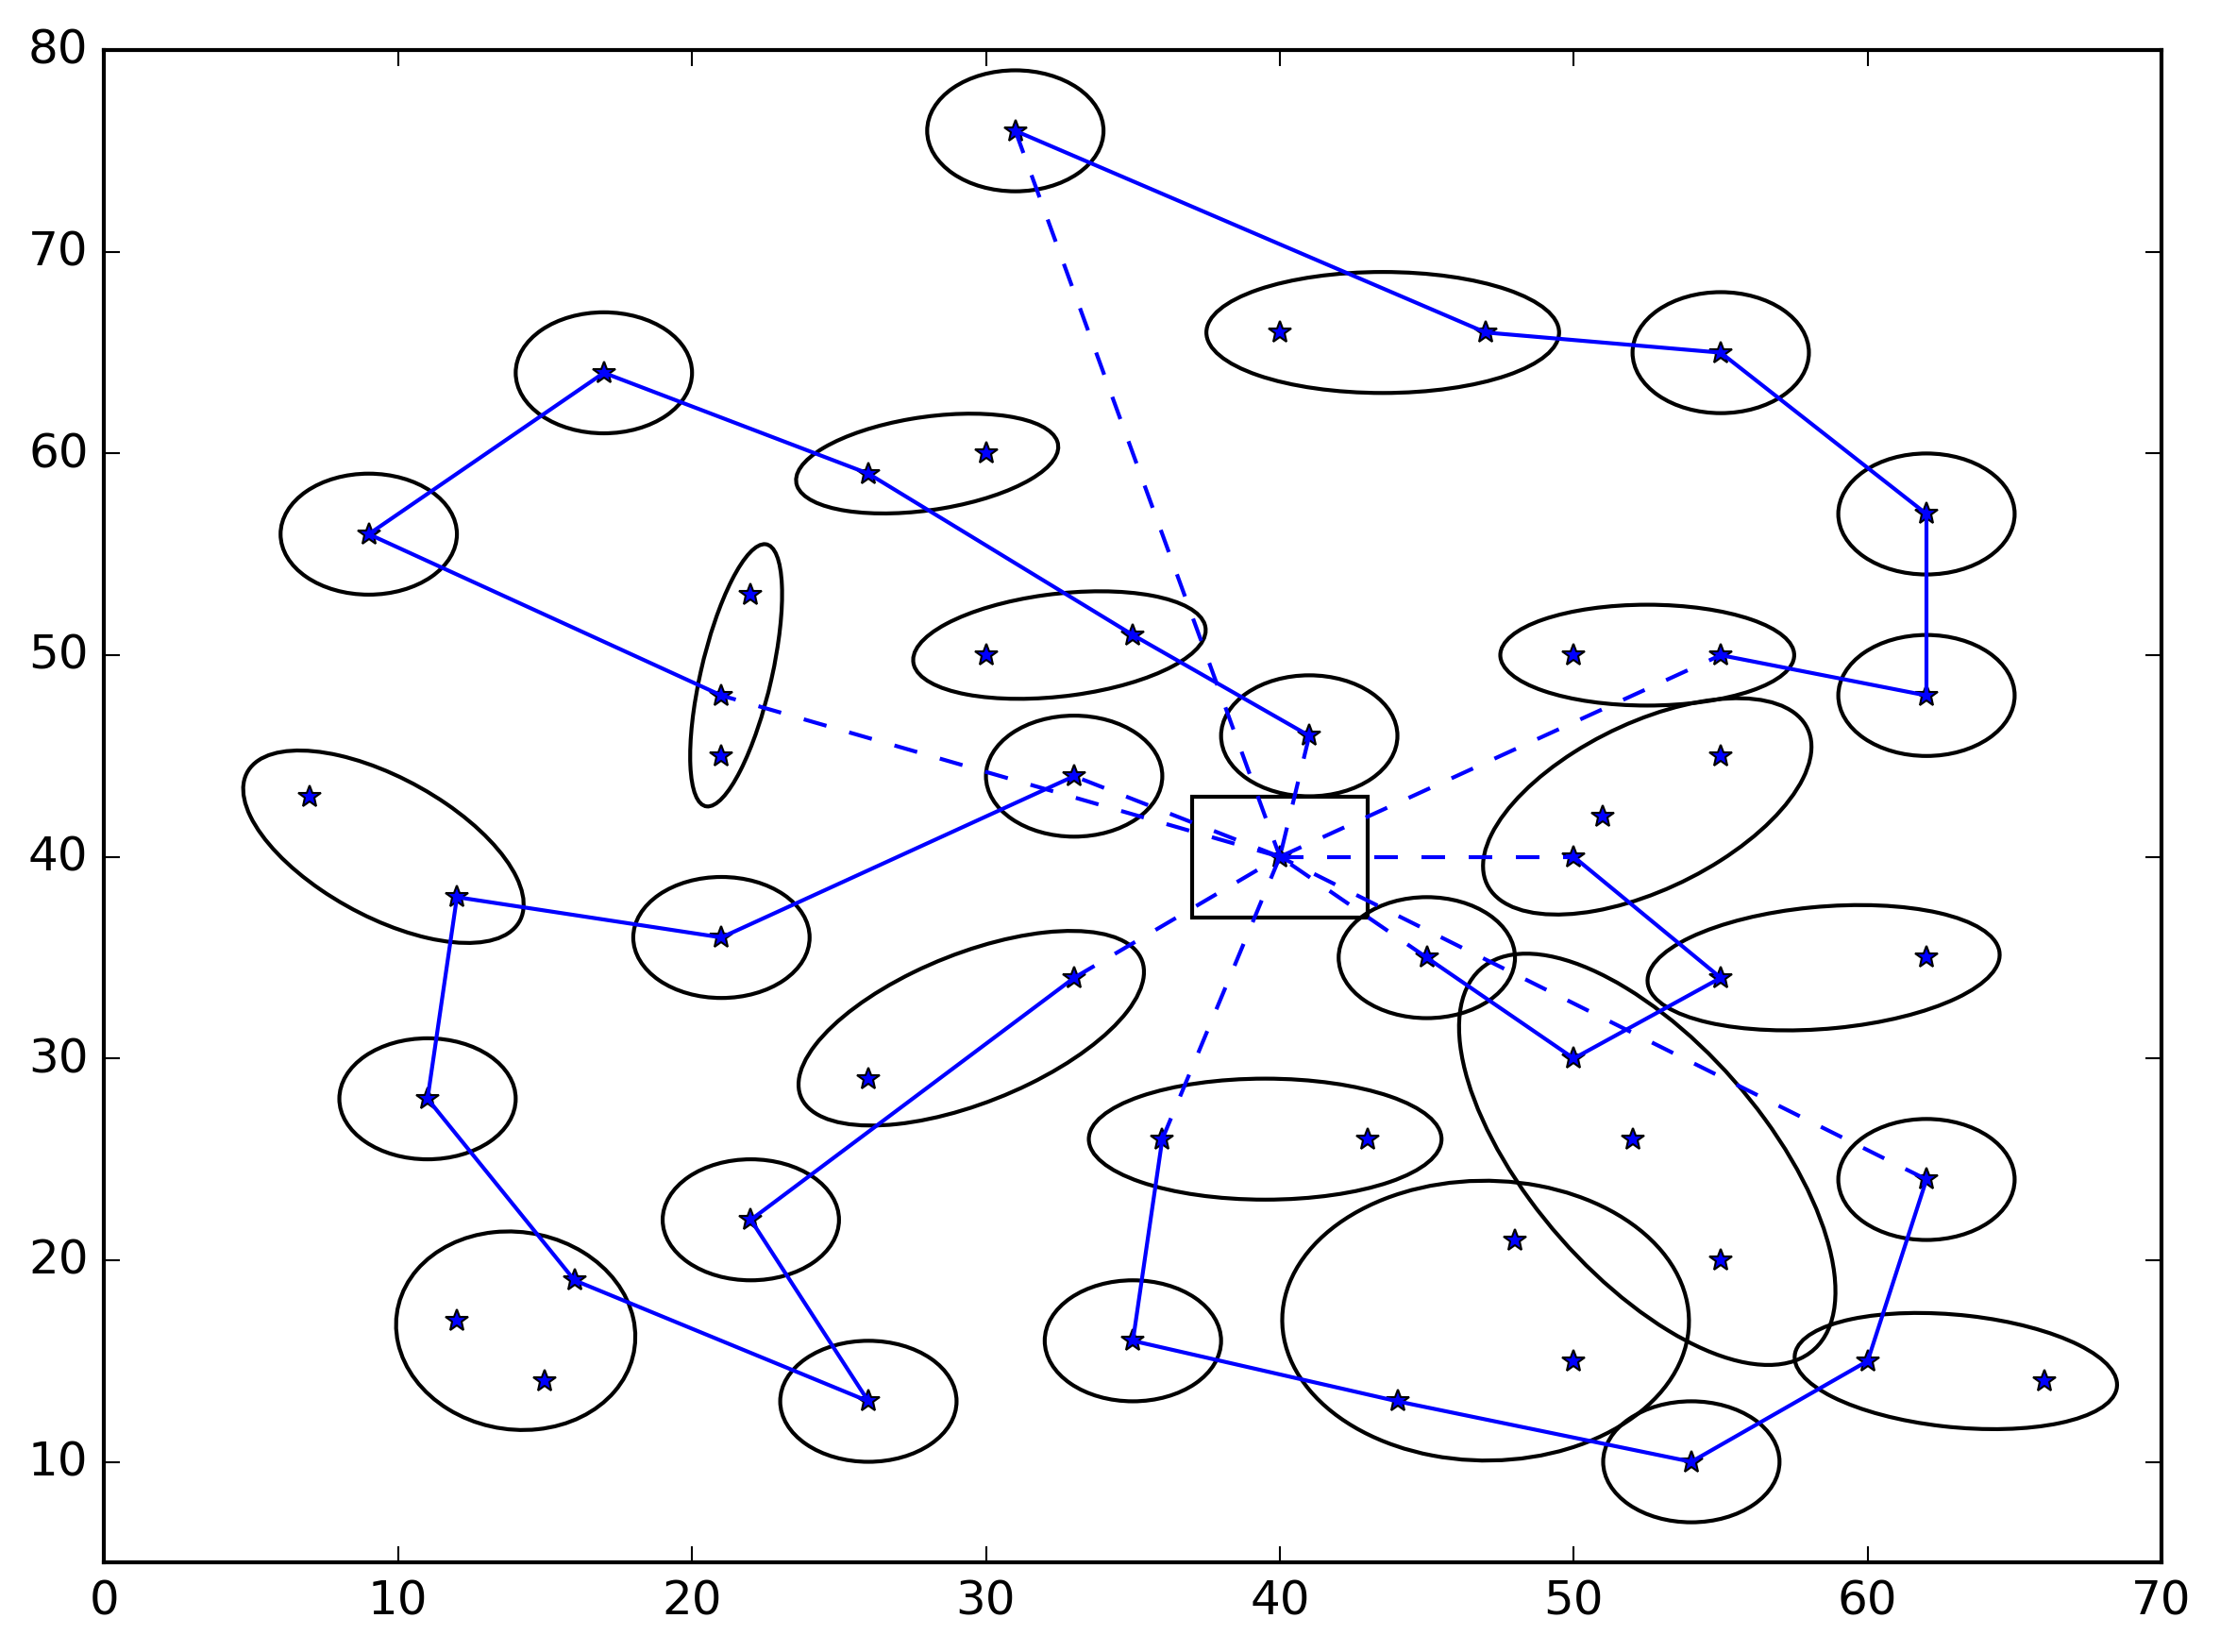
\includegraphics[width=\linewidth]{Images/P-n50-k10-c30_flow_n50_k31_m5_Q200_TL150_optimum.png}
\caption{\texttt{P-n50-k10}}
\end{figure}

\column{.33\textwidth}
\begin{figure}
\centering
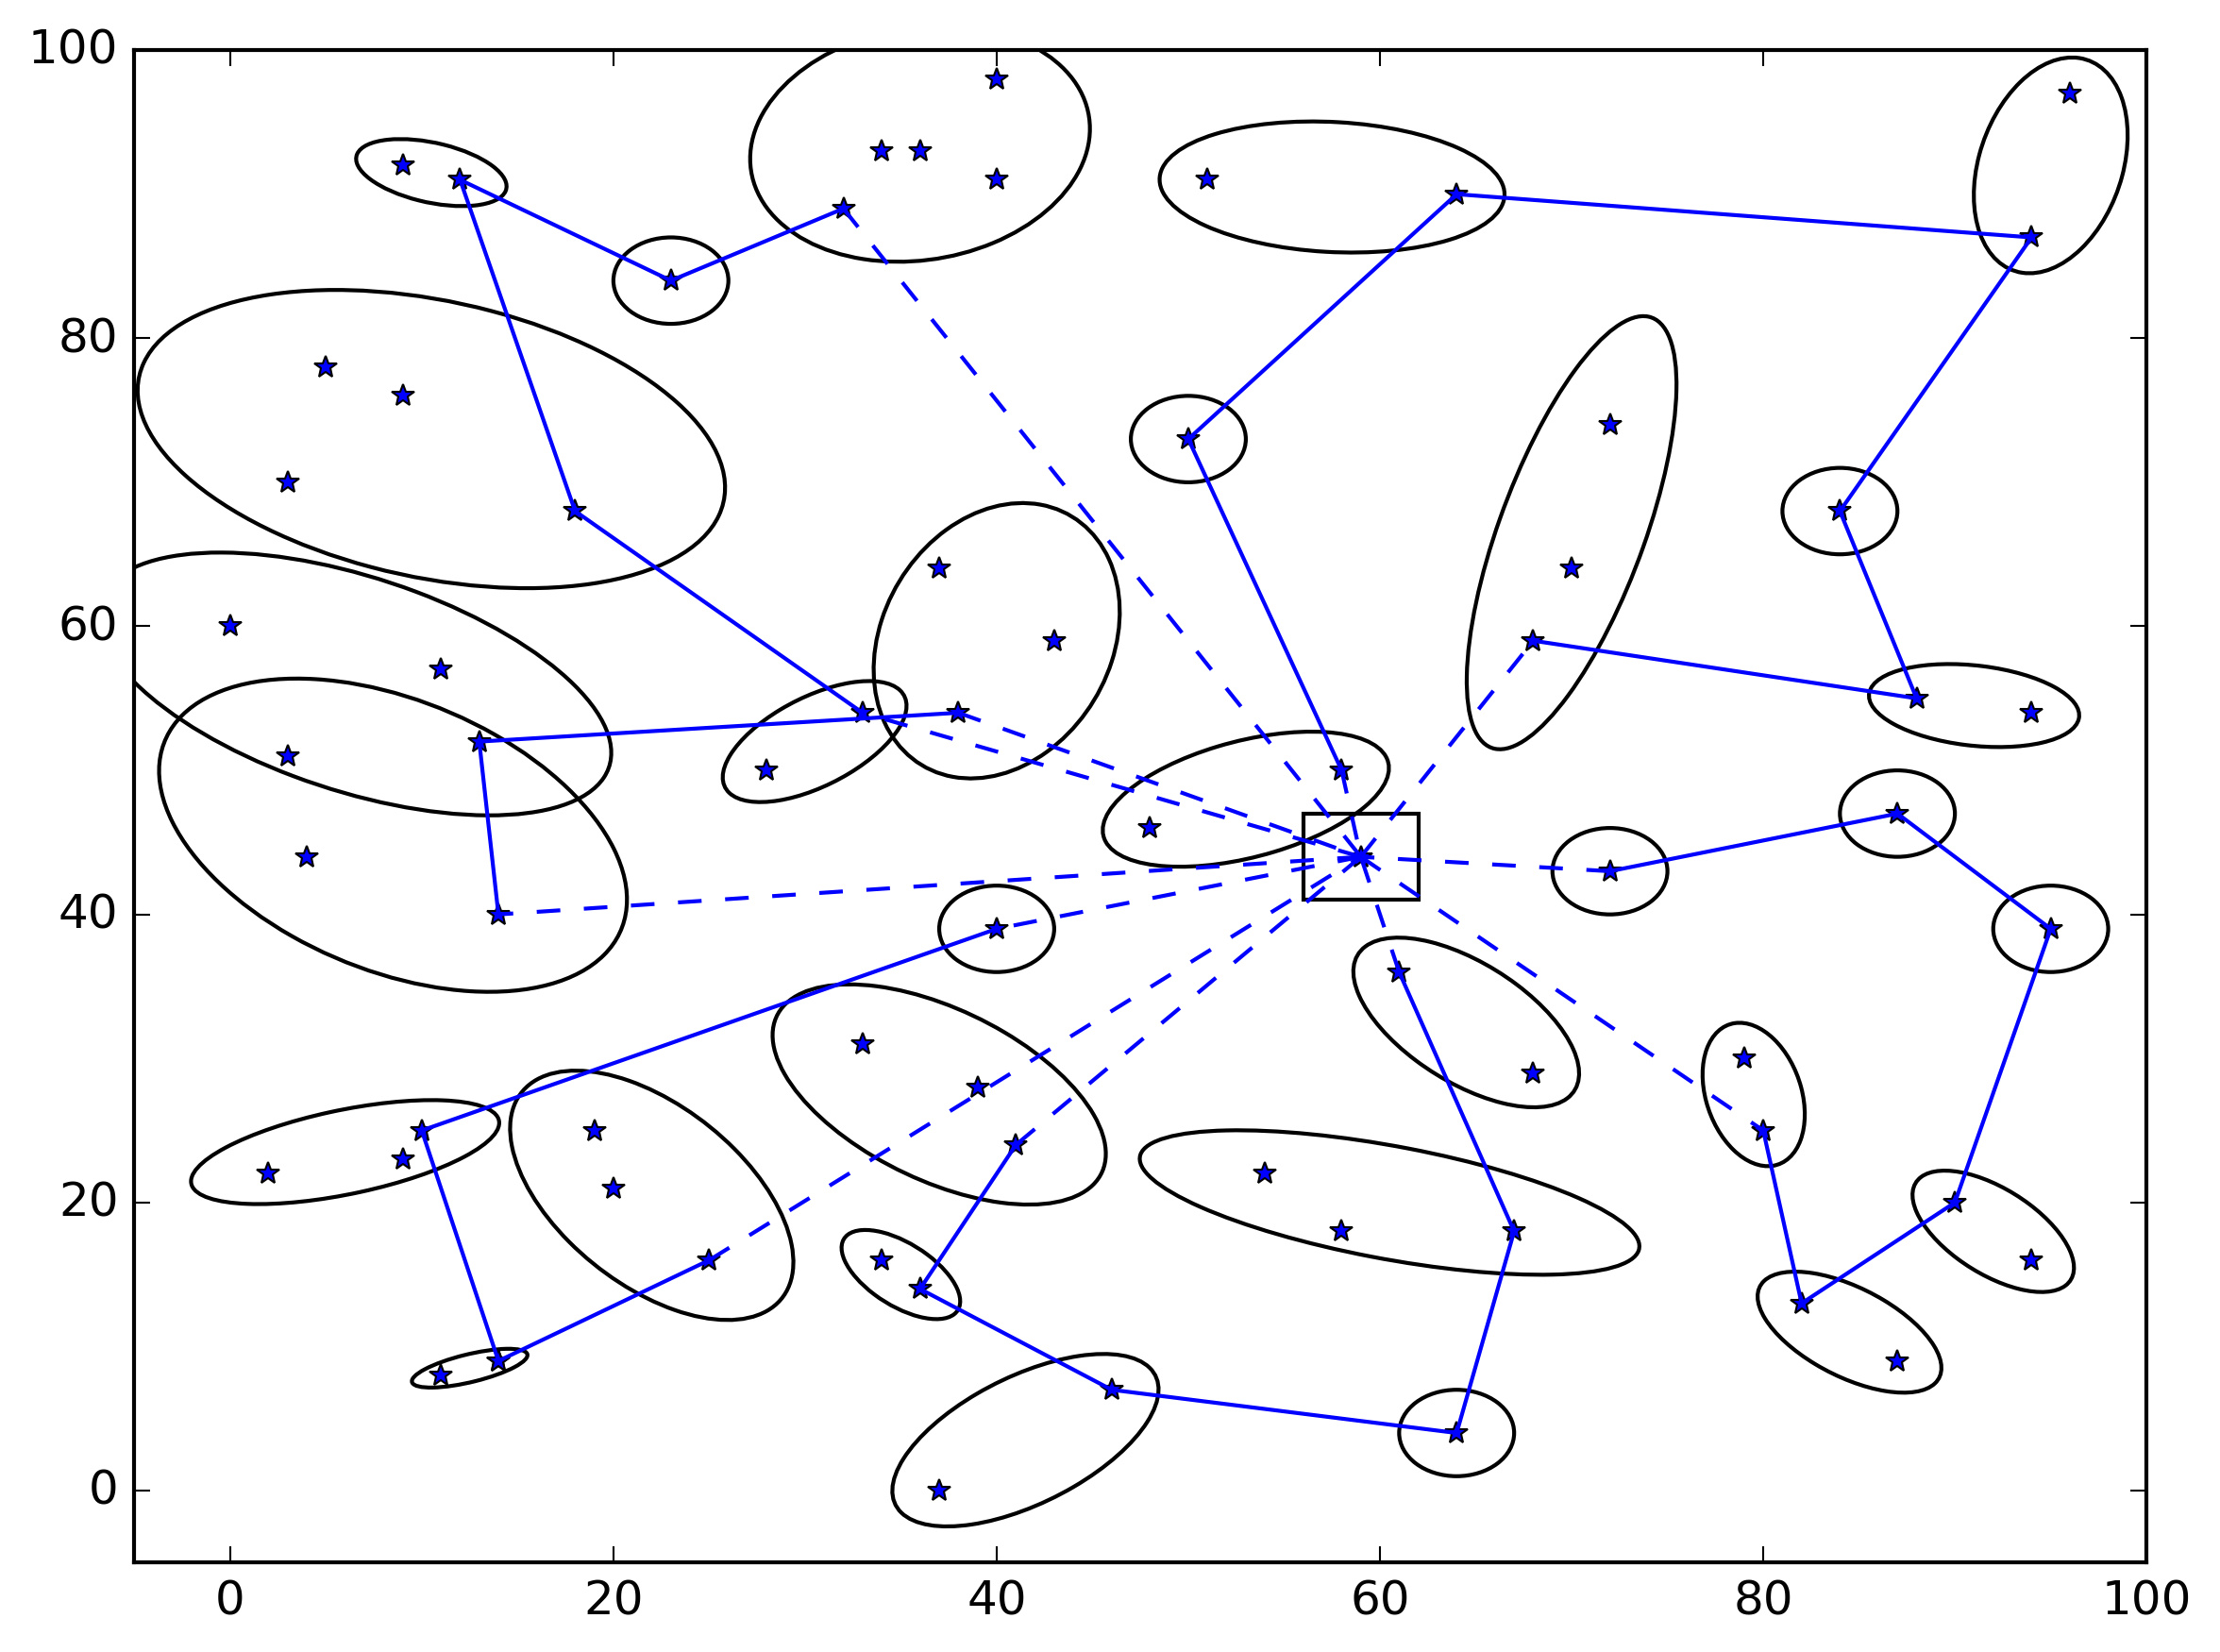
\includegraphics[width=\linewidth]{Images/A-n69-k9-c31_flow_n69_k32_m6_Q150_TL240_map.png}
\caption{\texttt{A-n69-k9}}
\end{figure}

\column{.33\textwidth}

\begin{figure}
\centering
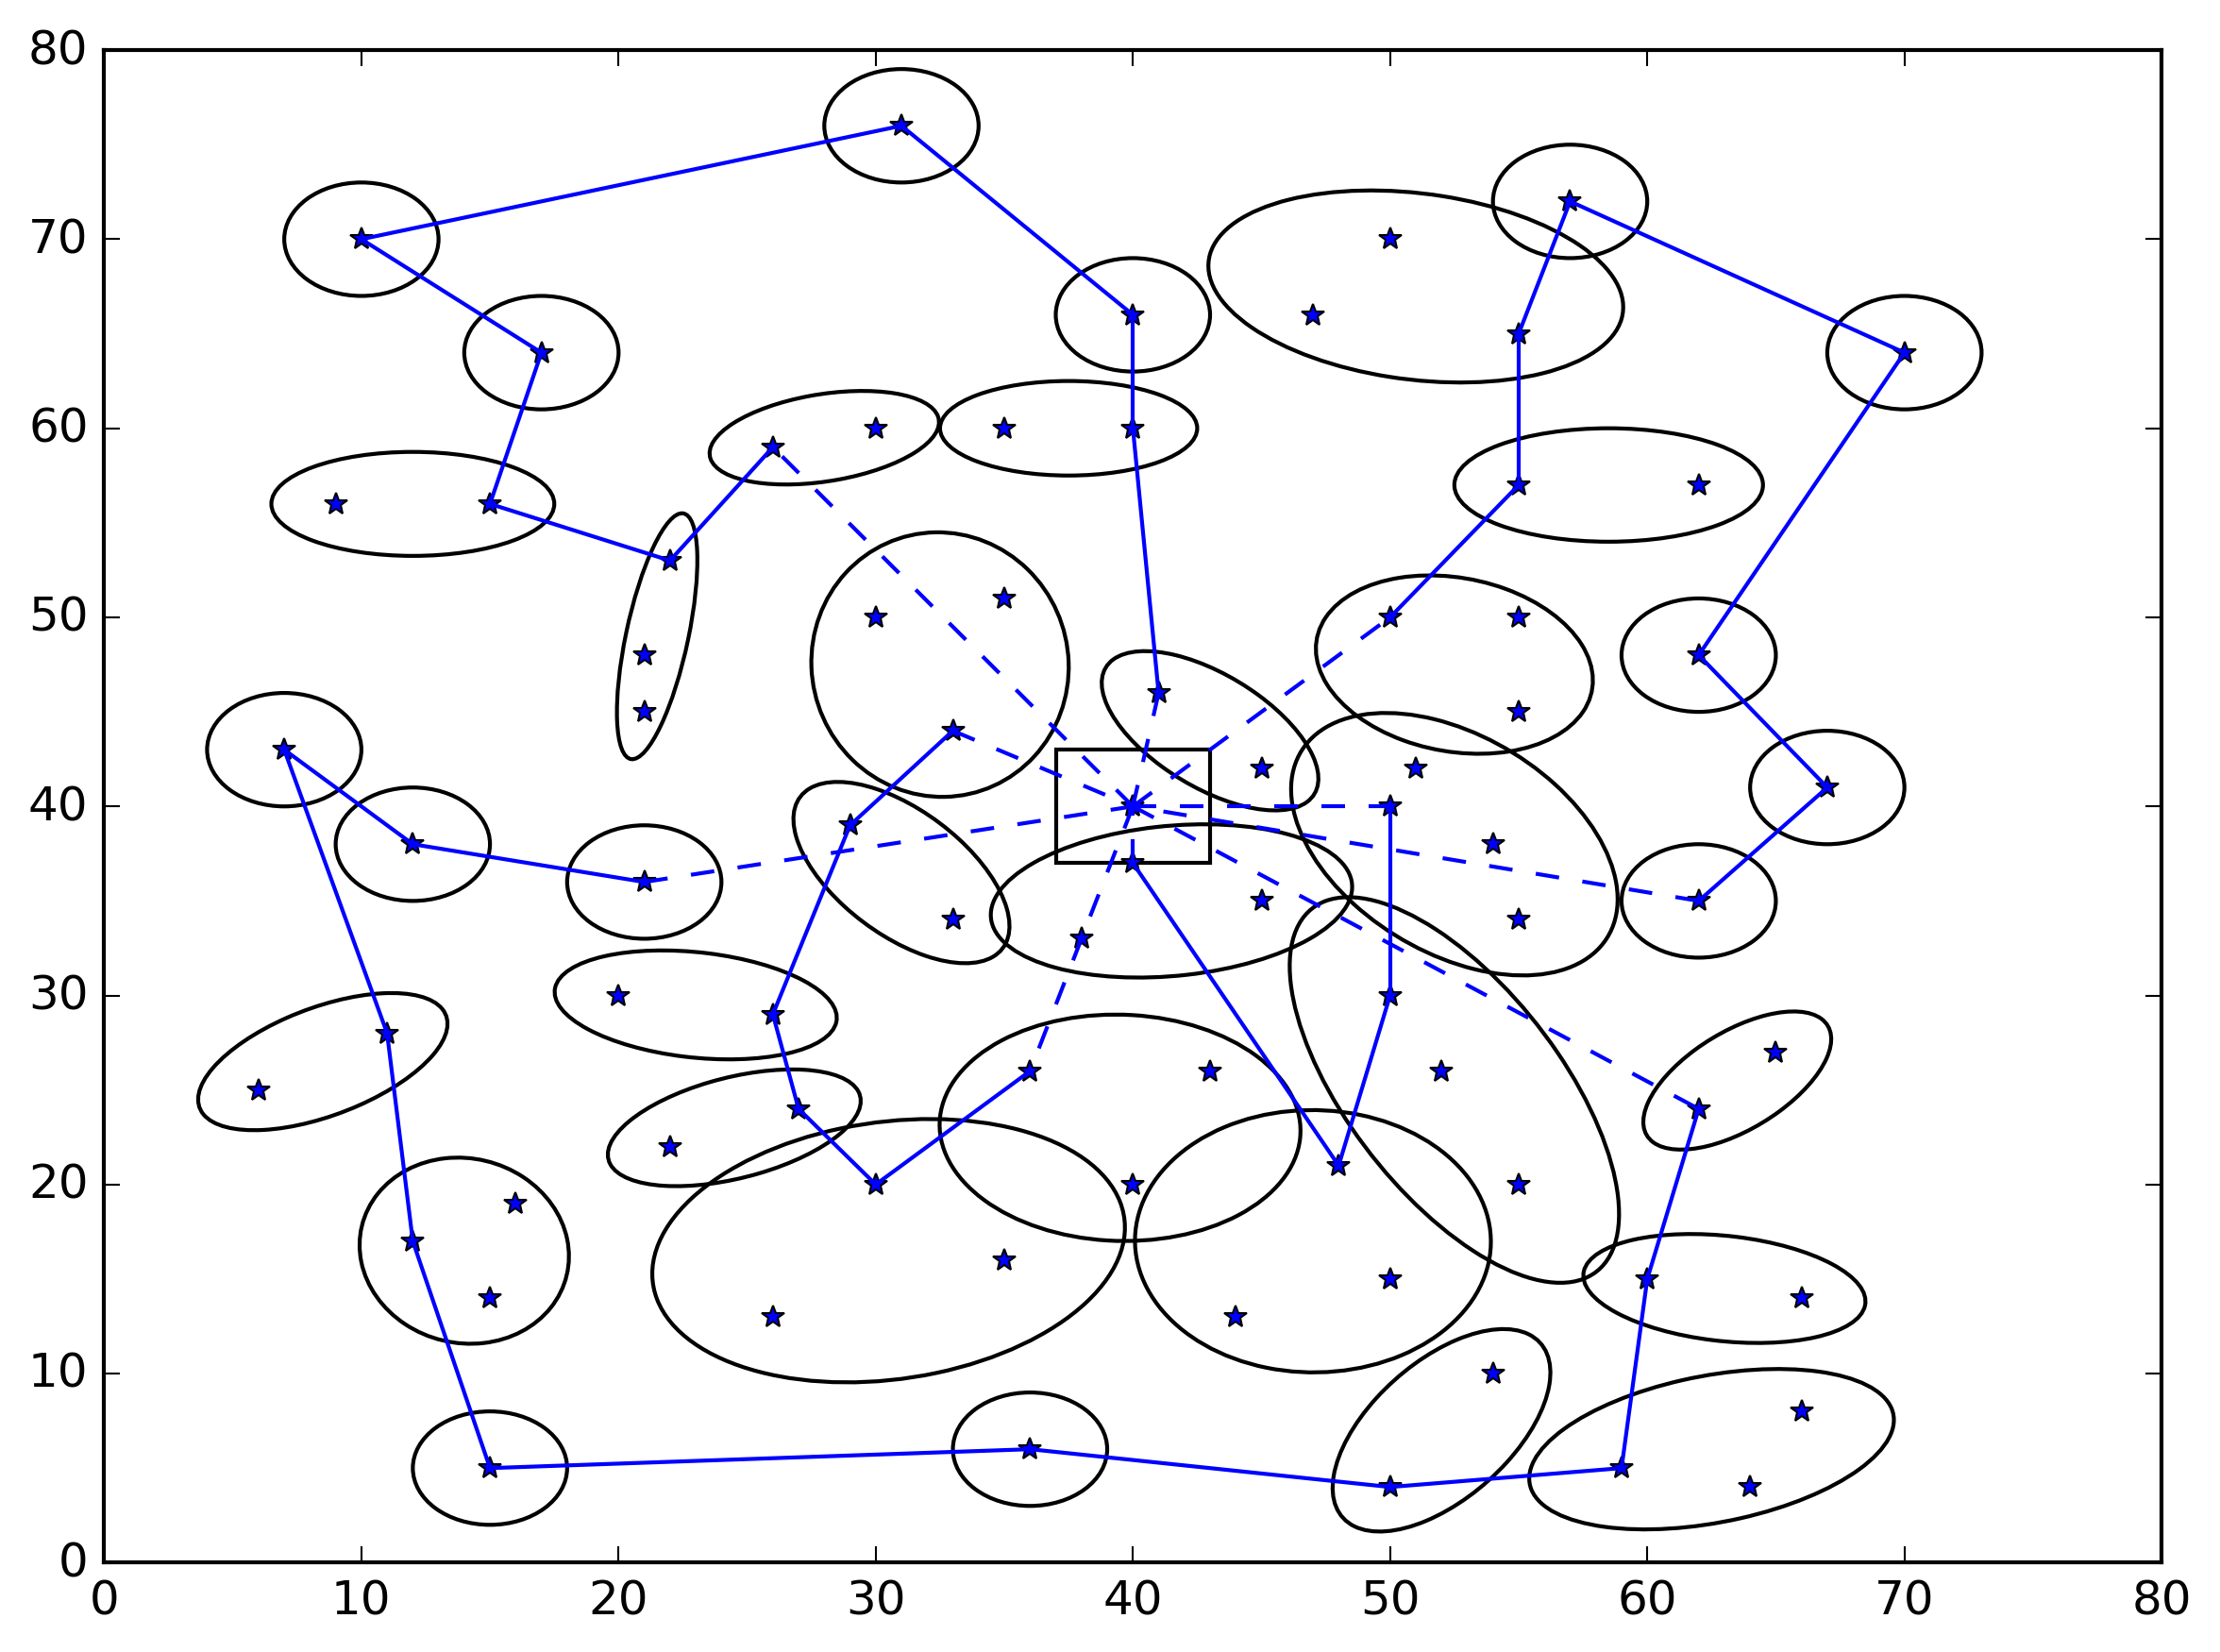
\includegraphics[width=\linewidth]{Images/P-n76-k5-c38_flow_n76_k39_m5_Q280_TL480_map.png}
\caption{\texttt{P-n76-k5}}
\end{figure}

\end{columns}
\end{frame}

\subsection{Root node relaxation}
\begin{frame}
\frametitle{\subsecname}
\begin{table}[htbp]
\centering
\caption{Deviation between root node relaxation and optimal values}
\label{tab:rootnode}
\resizebox{0.9\linewidth}{!}{
\begin{tabular}{@{}ccccc@{}}
\toprule
\textbf{Instance}              & \textbf{\begin{tabular}[c]{@{}c@{}}Best known\\  objective\end{tabular}} & \textbf{Formulation} & \textbf{\begin{tabular}[c]{@{}c@{}}Root node\\   relaxation\end{tabular}} & \textbf{\% Deviation} \\ \midrule
\texttt{GVRP1}          & 527.813     & flow                 & 498.594                        & 5.54                  \\
                               &                              & node                 & 449.358                       & 14.86                 \\ \midrule
\texttt{GVRP2}         & 557.564     & flow                 & 533.9                       & 4.24                  \\
                               &                              & node                 & 545.365                       & 2.19                  \\ \midrule
\texttt{P-n50-k10} & 417.742     & flow                 & 384.597  & 7.93                  \\
                               &                              & node                 & 338.098                       & 19.07	  \\ \midrule
\texttt{A-n69-k9}  & 756.131     & flow                 & 692.212 & 8.45                  \\
                               &                              & node                 & 560.44                       & 25.88 \\ \midrule
\texttt{P-n76-k5}  & 500.955     & flow                 & 450.746                       & 11.27                 \\
                               &                              & node                 & 399.788                        & 21.30                 \\ \bottomrule
\end{tabular}
}
\end{table}
\end{frame}

\subsection{Model comparision}

\begin{frame}
\frametitle{\subsecname}
\begin{table}[htbp]
\centering
\caption{Model comparision for GVRP instances (time limit = 1 hour)}
\label{tab:compstudy}
\resizebox{0.9\linewidth}{!}{
\begin{tabular}{@{}cccccc@{}}
\toprule
\textbf{Instance}              & \textbf{Formulation} & \textbf{Status} & \textbf{\begin{tabular}[c]{@{}c@{}}Objective\\   value\end{tabular}} & \textbf{\begin{tabular}[c]{@{}c@{}}Relative gap\\   (\%)\end{tabular}} & \textbf{\begin{tabular}[c]{@{}c@{}}Number \\ of constraints\end{tabular}} \\ \midrule
\texttt{GVRP1}         & flow                 & Optimal         & 527.813            & 0.01                       & 2108                 \\
                               & node                 & Feasible        & 527.813            & 5.42                       & 1482                 \\ \midrule
\texttt{GVRP2}         & flow                 & Optimal         & 557.564            & 0.00                       & 1242                 \\
                               & node                 & Optimal         & 557.564            & 0.00                       & 952                  \\ \midrule
\texttt{P-n50-k10} & flow                 & Feasible        & 417.742            & 0.75                       & 3094                 \\
                               & node                 & Feasible        & 417.742            & 14.69                      & 2132                 \\ \midrule
\texttt{A-n69-k9}  & flow                 & Feasible        & 756.131            & 1.25                       & 3385                 \\
                               & node                 & Feasible        & 763.045            & 18.59                      & 2360                 \\ \midrule
\texttt{P-n76-k5}  & flow                 & Feasible        & 508.194            & 6.04                       & 4896                 \\
                               & node                 & Feasible        & 595.149            & 31.20                      & 3374                 \\ \bottomrule
\end{tabular}
}
\end{table}
\end{frame}
\subsection{Outcomes}
\begin{frame}
\frametitle{\subsecname}
\begin{itemize}
\item New test cases represent more realistic benchmark instances for GVRP because of non-unit customer demands
\item Zero-gap solutions found for two out of three new test cases
\item Flow-based formulation outperforms node-based 
\item Formulations scale with number of customers rather than number of clusters
\end{itemize}
\end{frame}

\begin{frame}[noframenumbering]
\Huge Thank you
\end{frame}

\begin{frame}[noframenumbering]
\frametitle{Key features \& assumptions}
\begin{itemize}
\item The total demand of each cluster can be satisfied via any of its nodes
\item The demand of each cluster $q_k$ is the sum of demands of each customer in cluster $k$
\item All vehicles are identical i.e. each vehicle has the same capacity $Q$
\item NP-hard because it includes the generalized traveling salesman problem as a special case when m = 1 and Q = $\infty$
\end{itemize}
\end{frame}

\begin{frame}[noframenumbering]
\begin{table}
\centering
\caption{Details of GVRPs}
\label{tab:problemdetails}
\resizebox{\linewidth}{!}{
\begin{tabular}{@{}cccccc@{}}
\toprule
\textbf{Instance} & \textbf{Customers} & \textbf{Clusters} & \textbf{Vehicles} & \textbf{Capacity} & \textbf{\begin{tabular}[c]{@{}c@{}}Total\\   demand\end{tabular}} \\ \midrule
\texttt{GVRP1}             & 50                 & 24                & 4                 & 15                & 50                                                                \\
\texttt{GVRP2}             & 60                 & 16                & 6                 & 15                & 60                                                                \\
\texttt{P-n50-k10}     & 49                 & 30                & 5                 & 200               & 951                                                               \\
\texttt{A-n69-k9}      & 68                 & 31                & 6                 & 150               & 845                                                               \\
\texttt{P-n76-k5}      & 75                 & 38                & 5                 & 280               & 1364                                                              \\ \bottomrule
\end{tabular}}
\end{table}
\end{frame}

\begin{frame}[noframenumbering]
\frametitle{General formulation}
\textbf{Sets}
\begin{itemize}
\item $V = \{0, 1, 2, ..., n\}$ set of customers
\item $K = \{0, 1, 2, ..., k\}$ set of clusters
\item $A = \{(i,j)|\; i,j\in V, i\ne j\}$ set of arcs (routes).
\end{itemize}
\textbf{Parameters}
\begin{itemize}
\item $c_{ij}$ is the cost of traveling from node $i$ to node $j$
\item $d_i$ is the demand of customer $i$
\item $q_r = \sum_{i \in V_r} d_i$, $r \in K$ is the demand of the cluster $V_r$
\item $M = \{1, \ldots,m\}$ set of identical vehicles
\item $Q$ is the capacity of each vehicle
\end{itemize}
\end{frame}
\end{document}